\documentclass{thuemp}
\usepackage{graphicx} 
\begin{document}

% 标题,作者
\emptitle{基于多模型融合的个人信贷违约风险预测研究}
\empauthor{许桐恺}{黄婧}{魏振邦}

% 奇数页页眉 % 请在这里写出第一作者以及论文题目
\fancyhead[CO]{{\footnotesize 许桐恺,黄婧,魏振邦: 基于多模型融合的个人信贷违约风险预测研究}}


%%%%%%%%%%%%%%%%%%%%%%%%%%%%%%%%%%%%%%%%%%%%%%%%%%%%%%%%%%%%%%%%
% 关键词 摘要 首页脚注      
%%%%%%%%关键词
\Keyword{信贷风控;违约预测;特征工程;梯度提升树;模型融合;Stacking}  


\maketitle

%%%%%%%%摘要
\begin{empAbstract}
在普惠金融加速发展的背景下,个人信贷业务快速增长,违约风险问题日益突出,亟需高效精准的风险预测模型。本文提出一套融合深度特征工程与多模型集成的端到端预测框架。通过系统预处理与多维特征构建,重点引入群体统计量与三阶共现特征刻画个体差异;建模阶段,采用 LightGBM 进行特征筛选,并基于 Optuna 优化 XGBoost、LightGBM 和 CatBoost 三个 GBDT 模型,最终以逻辑回归为元模型实现 Stacking 融合。实验证明,融合模型在验证集上 AUC 达 0.7400,天池排行榜排名第 43(截至 2025 年 6 月 11 日),显著优于单一模型。研究验证了特征构建与模型融合在信贷风控中的关键价值,具备良好应用前景。 
\end{empAbstract}

%%%%%%%%英文标题、作者、摘要、关键词
\KeywordEn{credit risk modeling; default prediction; feature engineering; gradient boosting decision trees; model ensembling; Stacking}
\emptitleEn{A Study on Personal Credit Default Risk Prediction Based on Multi-Model Ensemble Learning}
\empauthorEn{Tongkai Xu}{Jing Huang}{Zhenbang Wei}

\begin{empAbstractEn}
The rapid expansion of personal credit, driven by inclusive finance, has brought heightened attention to default risk, necessitating efficient risk prediction models. This paper introduces an end-to-end framework that merges deep feature engineering with a multi-model ensemble. The process involves systematic preprocessing and multi-dimensional feature construction, with a particular focus on integrating group statistics and third-order co-occurrence features. For modeling, LightGBM is used for feature selection, followed by Optuna-optimized XGBoost, LightGBM, and CatBoost models, which are then combined using a Stacking ensemble with logistic regression as the meta-model. Experimental results demonstrate that this integrated approach significantly outperforms single models, achieving an AUC of 0.7404 on the validation set and ranking 37th on the Tianchi Leaderboard as of June 8, 2025, thereby underscoring the critical value and promising application prospects of advanced feature construction and model fusion in credit risk control.

\end{empAbstractEn}

%%%%%%%%首页角注,依次为实验时间、报告时间、学号、email



%%%%%%%%!首页角注可能与正文重叠,请通过调整正文中第一页的\enlargethispage{-3.3cm}位置手动校准正文底部位置:
%%%%%%%%%%%%%%%%%%%%%%%%%%%%%%%%%%%%%%%%%%%%%%%%%%%%%%%%%%%%%%%%
%  正文由此开始
\wuhao 
%  分栏开始

\section{引~~言}
\enlargethispage{-3.3cm}
\subsection{研究背景与意义}
近年来,随着数字技术与金融服务的深度融合,普惠金融 (Inclusive Finance) 在全球范围内以前所未有的速度加速发展。作为其核心业务之一,个人信贷服务极大地拓宽了金融服务的覆盖面,为个人消费者和小型企业主提供了重要的资金支持,有效促进了消费升级和实体经济的活力。然而,业务规模的迅速扩张也伴随着信用风险的显著增加。个人信贷违约事件不仅会给放贷机构带来直接的经济损失,还可能引发连锁反应,影响金融市场的稳定。因此,建立一套科学、精准、高效的个人信贷违约风险预测体系,已成为金融机构风险管理部门乃至整个金融行业亟待解决的核心问题。

传统的信贷风控主要依赖于基于专家规则和以逻辑回归为代表的线性模型构建的信用评分卡 \citep{siddiqi1997statistical}。这类方法虽然具有良好的解释性和稳定性,但在处理高维度、非线性、强交互的现代信贷数据时,其预测能力的局限性日益凸显。随着大数据和人工智能技术的进步,以梯度提升决策树 (Gradient Boosting Decision Tree, GBDT) 为代表的机器学习模型,如 XGBoost、LightGBM 和 CatBoost,因其强大的非线性拟合能力和出色的预测性能,已在信贷风控领域展现出巨大的应用潜力。如何充分利用这些先进模型,深度挖掘数据价值,构建性能更优越的预测模型,是本研究的出发点和核心目标。

\subsection{相关工作与文献综述}
信贷违约预测作为金融风控领域的经典问题,一直是学术界和工业界的研究热点。早期的研究主要集中于统计模型,其中 Altman 提出的 Z-Score 模型 \citep{altman1968financial} 和以逻辑回归 \citep{hosmer2013applied} 为基础的评分卡模型是里程碑式的成果,它们至今仍在许多金融机构的基准系统中使用。这些模型的优点在于结构简单、结果易于解释,但其线性的假设限制了它们从复杂数据中学习的能力。

进入21世纪,机器学习方法被广泛引入该领域。支持向量机 (SVM) \citep{cortes1995support}、神经网络 (Neural Networks) \citep{west2000neural} 和随机森林 (Random Forest) \citep{breiman2001random} 等模型在多个数据集上被证明优于传统统计模型。近年来,以 Friedman 提出的梯度提升机 \citep{friedman2001greedy} 为基础的集成学习算法,特别是其高效实现 XGBoost \citep{chen2016xgboost}、LightGBM \citep{ke2017lightgbm} 和 CatBoost \citep{prokhorenkova2018catboost},已成为处理表格类数据预测任务的“利器”。大量研究和数据竞赛实践(如 Kaggle)表明,这些 GBDT 模型在信贷风控任务中通常能取得顶尖的性能。

然而,先进的模型并不能自动保证最佳的结果。现代机器学习研究的共识是“数据和特征决定了机器学习的上限,而模型和算法只是逼近这个上限而已” \citep{ng2016nutshell}。因此,特征工程,即从原始数据中创造出对模型有价值的输入变量,被认为是提升模型性能的关键。同时,为了进一步突破单一模型的性能瓶颈,模型融合 (Model Ensembling) 技术,特别是 Stacking 堆叠融合 \citep{wolpert1992stacked},被证明是行之有效的策略。它通过训练一个“元模型”来智能地组合多个基模型的预测,从而获得比任何单一模型都更好的泛化能力。

\subsection{本文主要工作与贡献}
尽管已有大量研究将机器学习应用于信贷风控,但如何系统性地结合深度特征工程、自动化模型优化与高级模型融合策略,构建一个端到端的、可复现的高性能建模框架,仍是值得深入探索的方向。基于此,本文的主要工作与贡献如下:

\begin{itemize}
    \item 构建了多维度的深度特征工程体系:本文不仅处理了基础特征,还重点设计并实现了高阶交叉特征,特别是群体统计特征(如均值、标准差、分位数等)和多阶共现次数特征,旨在从数据的交互中捕捉更深层次的、具有业务含义的风险模式。
    \item 实践了科学的模型优化流程:本文采用基于 XGBoost 特征重要性的过滤法进行了高效的特征选择,并引入 Optuna 自动化调优框架,对 XGBoost、LightGBM、CatBoost 三个模型的超参数进行了系统性的贝叶斯优化,以寻求其最佳性能。
    \item 实现了有效的模型融合策略:本文对比了简单平均融合与基于逻辑回归元模型的 Stacking 堆叠融合两种策略。实验证明,Stacking 融合能够智能地组合不同基模型的优势,取得了最佳的预测性能。
    \item 提供了可复现的高性能基线:本文提出的端到端建模框架,在公开数据集上取得了 AUC 0.7400 的优异成绩,并获得了天池排行榜第 43 名(截至特定日期)的排名,为相关领域的研究和实践提供了强有力的性能基准和方法论参考。
\end{itemize}

\section{实验准备}
\subsection{数据初步分析与预处理}
\label{subsec:data_analysis_preprocessing}

本研究的数据分析与建模工作首先开展了系统性的探索性数据分析(Exploratory Data Analysis, EDA)与规范化的数据预处理操作,旨在深入理解变量内涵及其统计分布特征,识别并纠正缺失、异常与格式不一致等数据质量问题,从而构建一个结构完备、语义明确、可供模型直接调用的高质量数据集,为后续特征工程与建模优化提供坚实的数据基础。

\subsubsection{数据集概览与变量解析}

本项目所使用的数据集包含约 80 万条贷款记录,涵盖 47 个原始特征,全面表征借款人的人口统计属性、财务状况、信用历史以及贷款申请的核心信息。根据变量的业务属性与结构特征,可将其划分为如下几类:

\begin{table}[H]
\centering
\caption{变量分类与说明}
% 使用 tabularx 环境,宽度为页面文本宽度 \textwidth
% X 列类型会自动伸缩,>{\raggedright\arraybackslash} 让长文本左对齐
\begin{tabularx}{\textwidth}{|l|p{4cm}|>{\raggedright\arraybackslash}X|}
\hline
类别 & 变量 & 描述 \\ \hline
标识信息 & \texttt{id} & 贷款记录唯一标识符 \\ \hline
贷款基本属性 & \texttt{loanAmnt}, \texttt{term}, \texttt{interestRate}, \texttt{installment}, \texttt{grade}, \texttt{subGrade} & 贷款金额、期限、利率、月供、信用等级 \\ \hline
借款人信息 & \texttt{employmentTitle}, \texttt{employmentLength}, \texttt{homeOwnership}, \texttt{annualIncome}, \texttt{verificationStatus} & 就业信息、房产状况、年收入及验证状态 \\ \hline
贷款目的与状态 & \texttt{purpose}, \texttt{title}, \texttt{initialListStatus}, \texttt{applicationType}, \texttt{policyCode} & 贷款用途、申请类型及列表状态等 \\ \hline
地理位置变量 & \texttt{postCode}, \texttt{regionCode} & 借款人所在地区信息 \\ \hline
信用行为与历史 & \texttt{dti}, \texttt{delinquency\_2years}, \texttt{ficoRangeLow}, \texttt{ficoRangeHigh}, \texttt{openAcc}, \texttt{pubRec}, \texttt{pubRecBankruptcies}, \texttt{revolBal}, \texttt{revolUtil}, \texttt{totalAcc}, \texttt{issueDate}, \texttt{earliesCreditLine} & 债务水平、信用账户状况及信用记录 \\ \hline
匿名化变量 & \texttt{n0}--\texttt{n14} & 经脱敏处理的行为特征变量 \\ \hline
目标变量 & \texttt{isDefault} & 贷款违约标记(1 表示违约,0 表示正常还款) \\ \hline
\end{tabularx}
\end{table}

\paragraph{(1)缺失值处理}

\begin{itemize}
  \item \textbf{数值型变量填充}:针对所有数值型特征(含匿名变量),采用固定值 \texttt{-999} 进行填充。此类极端值设计可被树模型有效识别为“缺失模式”的代理变量,便于建模捕捉其潜在信息。
  \item \textbf{分类变量填充}:对于类别变量,统一使用占位符\texttt{MISSING}进行填充。
\end{itemize}

\begin{figure}[H]
    \centering
    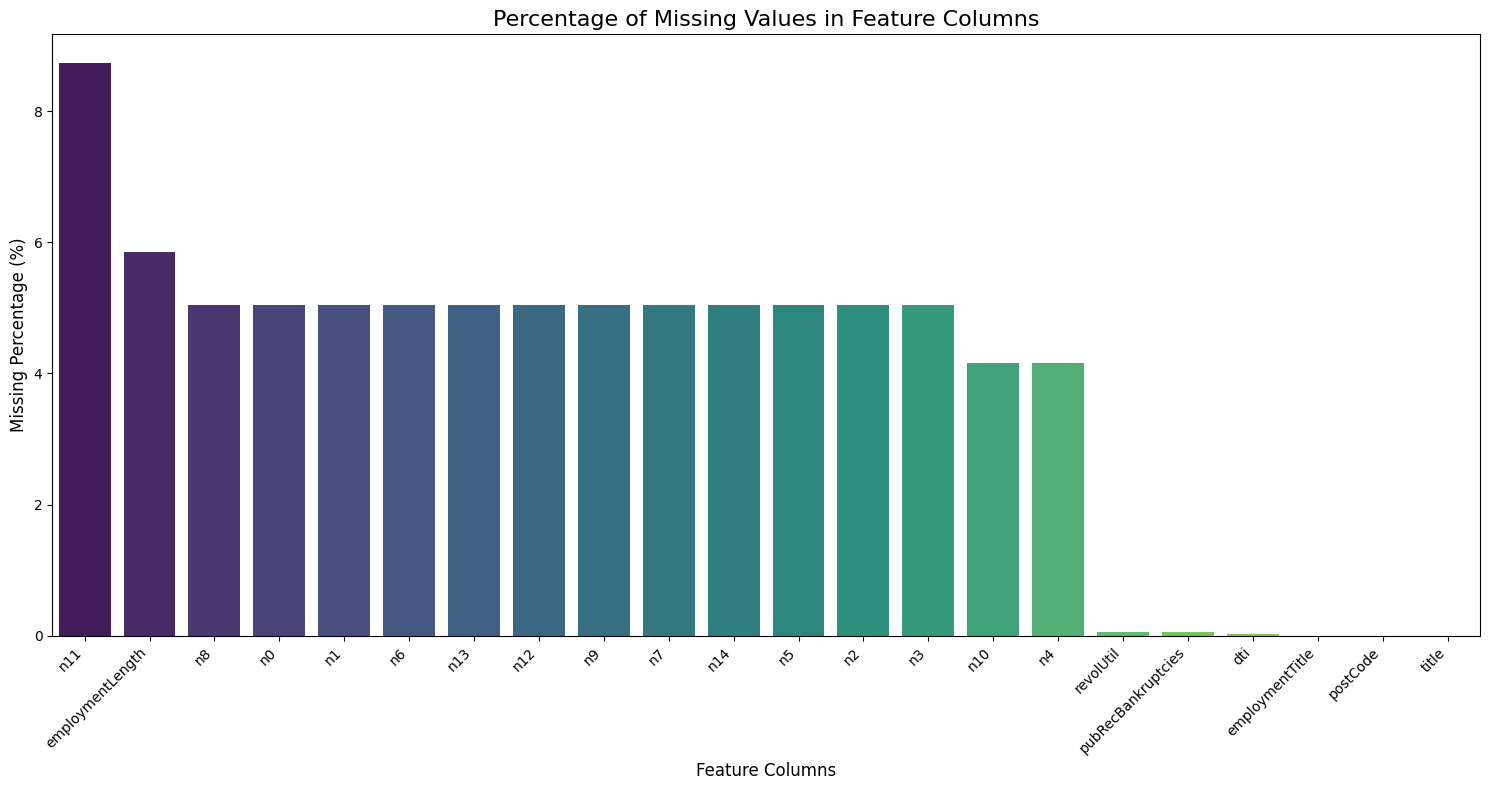
\includegraphics[width=0.8\textwidth]{image/results/__results___files/__results___9_1.png} % <-- 替换为你的图片路径
    \caption{数据集中特征缺失值百分比分布图}
    \label{fig:missing_values}
\end{figure}

\paragraph{(2)数据类型规范与变量编码}
\begin{itemize}
    \item \textbf{时间变量标准化}:将 \texttt{issueDate} 与 \texttt{earliesCreditLine} 自字符串格式转换为 \texttt{datetime64} 类型,便于后续构造衍生时间变量(如账户年龄、放款月份等)。
    \item \textbf{有序变量编码}:
    \begin{itemize}
        \item \texttt{grade}:将信用等级 \texttt{'A'}--\texttt{'G'} 编码为 \texttt{1}--\texttt{7},保留其单调顺序结构;
        \item \texttt{subGrade}:通过组合编码公式(如 \texttt{主等级值 \times 5 + 子等级编号}),实现主等级与子等级顺序的连续性表达;
        \item \texttt{employmentLength}:对就业年限中的模糊表达(如 \texttt{<1 year}, \texttt{10+ years})进行规则解析与清洗,统一转换为浮点数形式(\texttt{<1 year} 计作 \texttt{0.5},\texttt{>10 year} 计作 \texttt{12}),增强其数值可解释性与计算能力。
    \end{itemize}
    \item \textbf{目标编码}:对于名义类别特征(Nominal Categorical Features),尤其是唯一值众多的高基数特征(如 \texttt{postCode}, \texttt{employmentTitle}, \texttt{title}),简单的独热编码会导致维度灾难。为此,我们采用了目标编码(Target Encoding)策略,其核心思想是用类别对应的目标变量 \texttt{isDefault} 的均值(即该类别的平均违约率)来代替类别本身,生成与目标高度相关的数值特征。具体实施方法如下:
    \begin{itemize}
        \item \textbf{外部多种子循环}:为保证编码稳定性,交叉验证过程使用多个不同随机种子重复多次。
        \item \textbf{内部 K-Fold 划分}:在每个种子循环内,将训练集划分为 $K$ 个互斥子集(折),取 $K=5$。
        \item \textbf{折外计算}:对每一折进行编码时,使用其余 $K-1$ 折数据计算类别均值,确保训练样本的编码值不依赖其自身目标标签,防止数据泄露。
        \item \textbf{验证集与测试集处理}:使用训练集上计算的全局目标均值映射转换验证集和测试集。对于验证集中出现的新类别,填充训练集目标变量的全局均值。
    \end{itemize}
    目标编码的数学原理如下:设第 $j$ 个类别特征为 $x_j$,其取值集合为 $\mathcal{C}_j$,目标变量为 $y$,全局样本均值为:
    \[
    \mu = \mathbb{E}[y]
    \]
    在训练集上采用 $K$ 折交叉验证。第 $k$ 折中,训练集记为 $D_{\text{train}}^{(k)}$,验证集为 $D_{\text{val}}^{(k)}$。对每个类别 $c \in \mathcal{C}_j$,在第 $k$ 折的训练集上计算目标均值:
    \[
    \mu_j^{(k)}(c) = \frac{ \sum_{i \in D_{\text{train}}^{(k)}} \mathbf{1}(x_j^{(i)} = c) \cdot y^{(i)} }
                          { \sum_{i \in D_{\text{train}}^{(k)}} \mathbf{1}(x_j^{(i)} = c) }
    \]
    将该编码值赋给验证集中所有对应类别值的样本:
    \[
    x_{j,\text{target\_mean}}^{(i)} = 
    \begin{cases}
    \mu_j^{(k)}(x_j^{(i)}), & \text{if } x_j^{(i)} \in \mathcal{C}_j^{(k)} \\
    \mu, & \text{if } x_j^{(i)} \notin \mathcal{C}_j^{(k)}
    \end{cases}
    \quad \text{for } i \in D_{\text{val}}^{(k)}
    \]
    在验证集 $X_{\text{val}}$ 上的目标编码使用训练集整体估计:
    \[
    x_{j,\text{target\_mean}}^{(i)} = 
    \begin{cases}
    \mu_j(x_j^{(i)}), & \text{if } x_j^{(i)} \in \mathcal{C}_j \\
    \mu, & \text{otherwise}
    \end{cases}
    \quad \text{for } i \in X_{\text{val}}
    \]
    其中,训练集整体的目标均值映射为:
    \[
    \mu_j(c) = \frac{ \sum_{i \in X_{\text{train}}} \mathbf{1}(x_j^{(i)} = c) \cdot y^{(i)} }
                     { \sum_{i \in X_{\text{train}}} \mathbf{1}(x_j^{(i)} = c) }
    \]
    通过上述方法,特征 \texttt{homeOwnership}, \texttt{purpose}, \texttt{regionCode}, \texttt{postCode}, \texttt{employmentTitle}, \texttt{title} 等被转换为信息密集的数值特征,显著增强了模型的预测能力。
\end{itemize}

\vspace{0.5em}
综上,通过上述系统的预处理流程,原始数据集中的质量缺陷得以显著改善,最终构建出结构规范、数据完整、类型统一的高质量“干净数据集”。该数据基础不仅满足建模算法的输入要求,同时也为后续特征工程与模型迭代提供了可靠支撑。

\subsection{特征工程}
特征工程是构建高性能预测模型的基石,其核心在于从原始数据中提取并创造出能够最大化模型学习效能的特征。一个设计精良的特征体系不仅能提升模型的预测精度,还能增强其泛化能力和业务可解释性。在本研究中,我们针对信贷风控问题的特性,构建了一个多层次、多维度的特征体系。

首先,我们对几个核心的原始数值特征进行了分布分析,如图 \ref{fig:original_dist} 所示。

\begin{figure}[H]
    \centering
    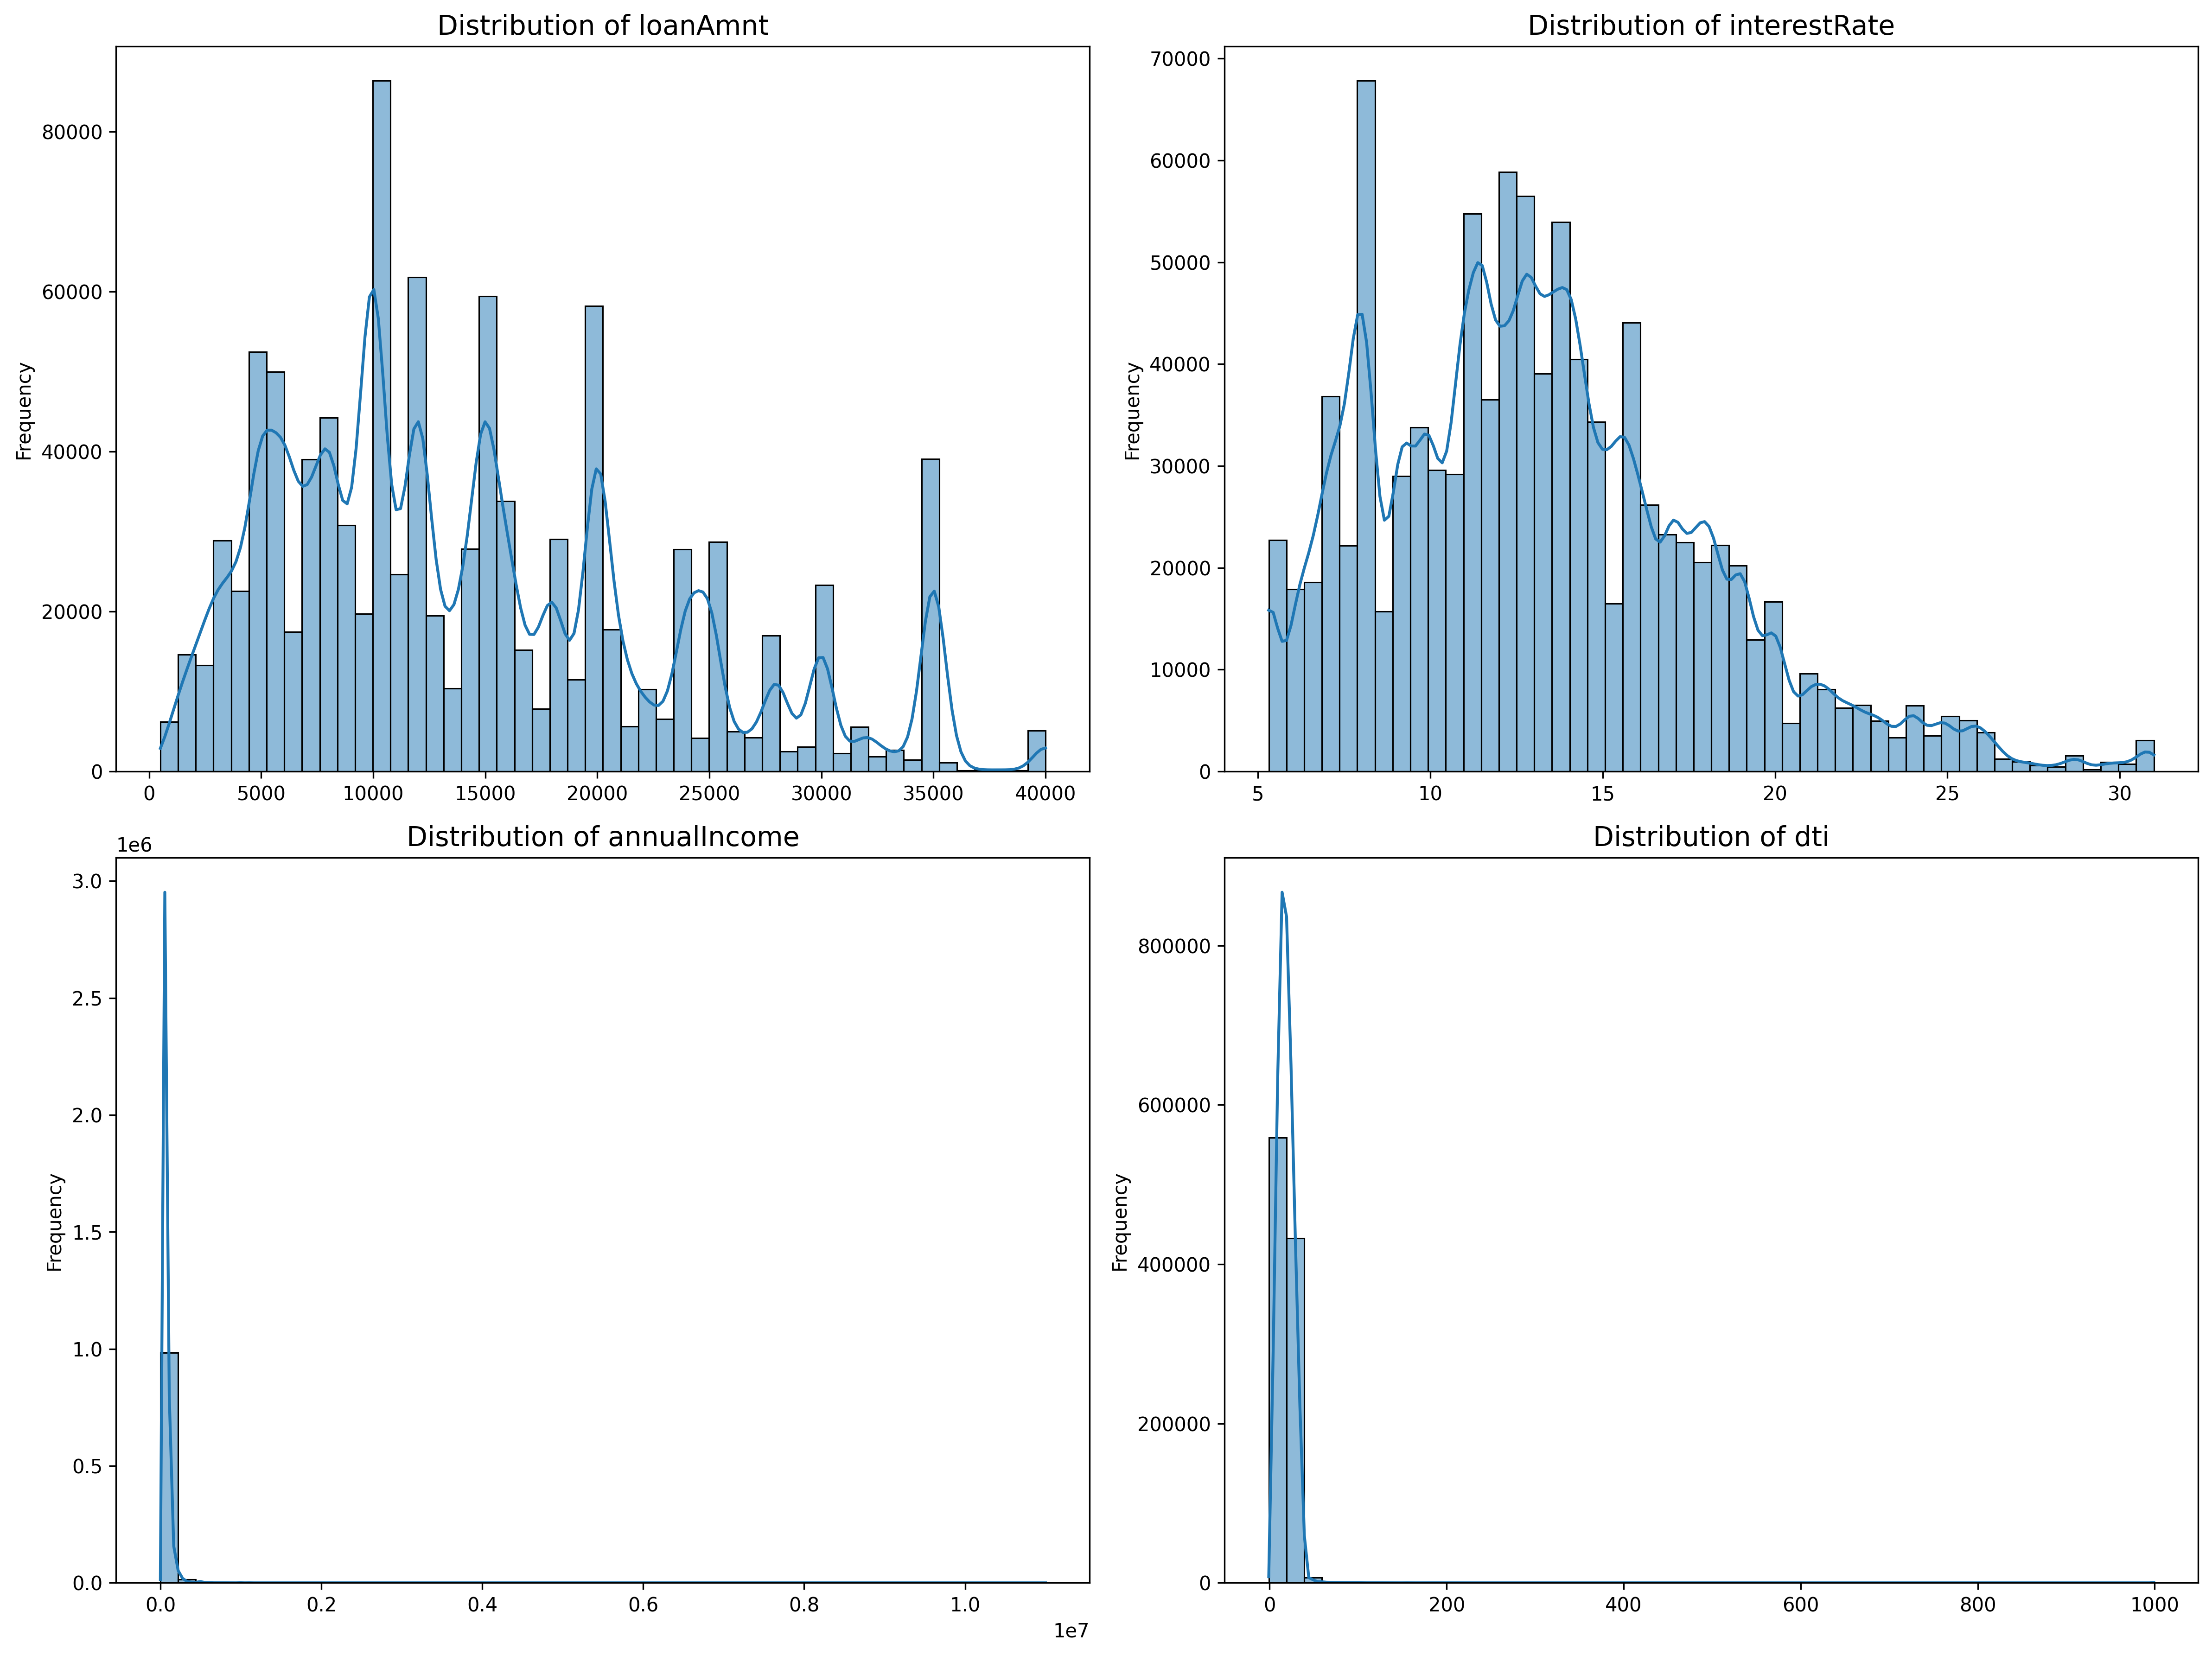
\includegraphics[width=0.8\textwidth]{image/results/images/major_Distribution.png} % <-- 替换为你的第一张图片路径
    \caption{原始关键数值特征的分布图}
    \label{fig:original_dist}
\end{figure}

从图 \ref{fig:original_dist} 中可以观察到几个重要的数据特性:\texttt{loanAmnt}(贷款金额)呈现出明显的多峰分布,这通常与标准化的贷款产品额度有关;\texttt{annualIncome}(年收入)和 \texttt{dti}(债务收入比)则表现为典型的严重右偏分布,其中包含了部分极端值。这些观察为我们后续进行对数变换等特征工程操作提供了依据。

% \begin{figure}[H]
%     \centering
%     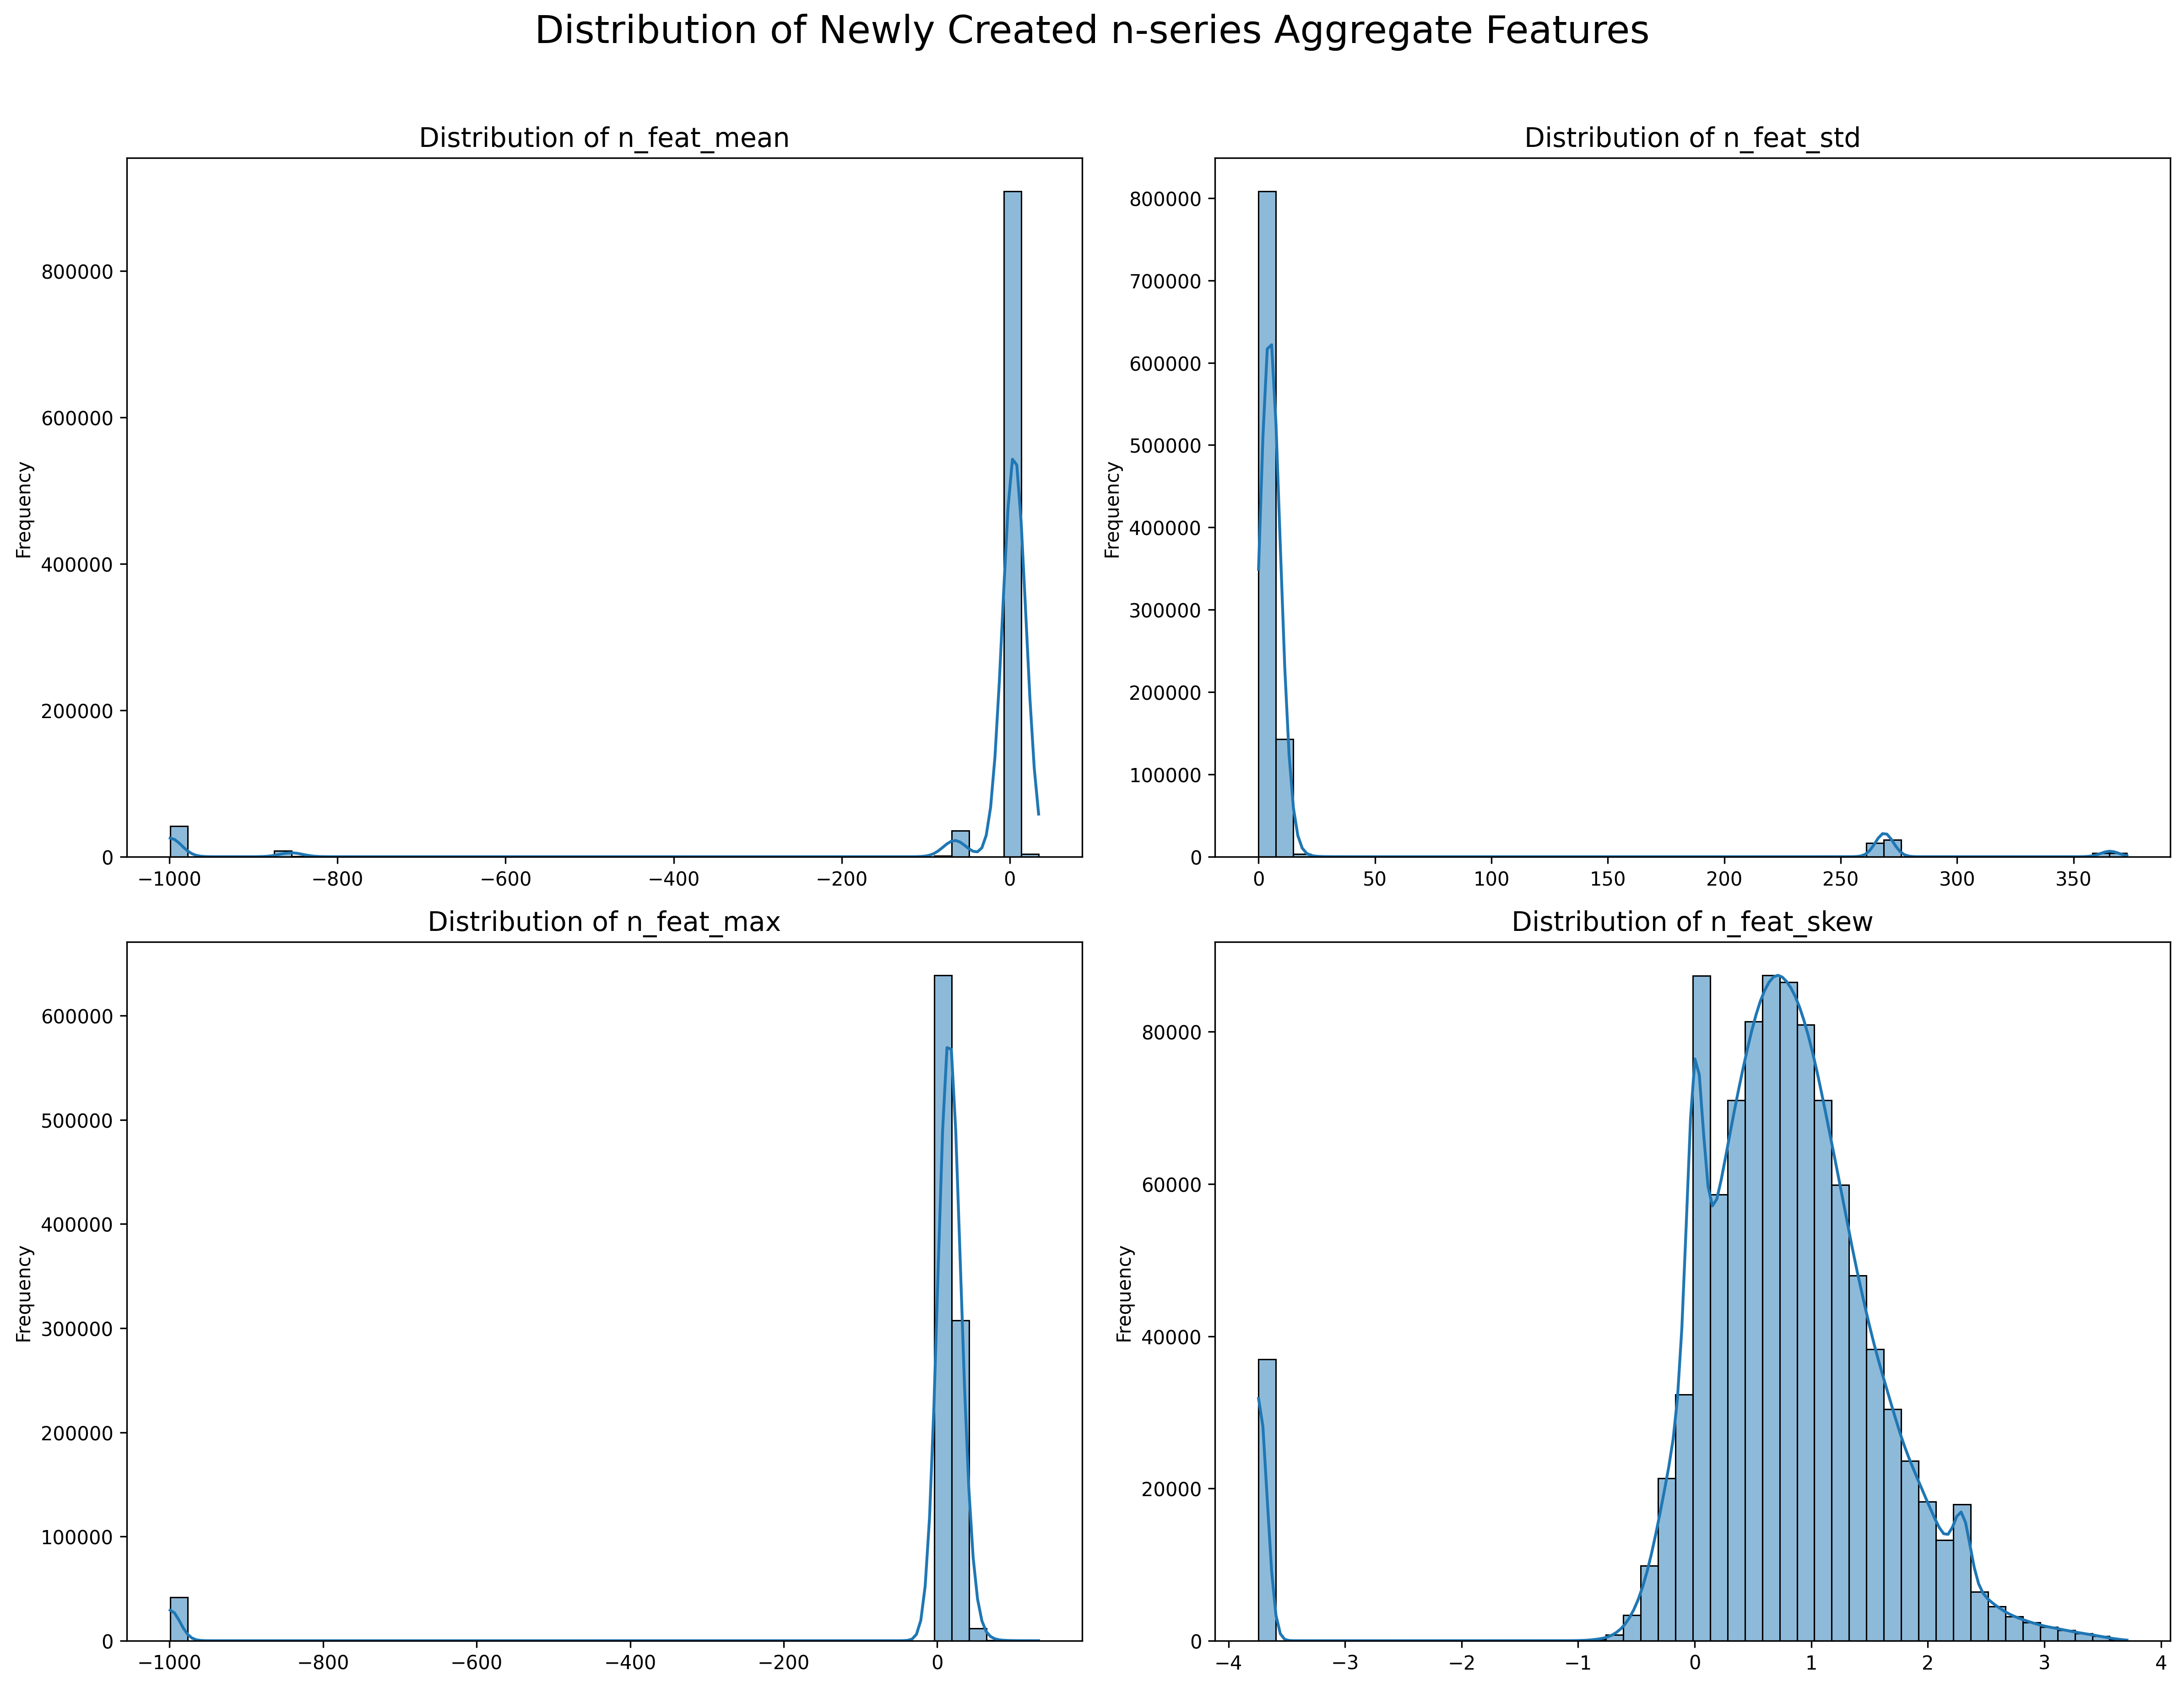
\includegraphics[width=0.9\textwidth]{image/results/images/n-series.png} % <-- 替换为你的第二张图片路径
%     \caption{新构造的 n 系列聚合特征的分布图}
%     \label{fig:n_agg_dist}
% \end{figure}
\subsubsection{\textbf{基础衍生特征}}

此阶段的目标是将原始数据转换为更具业务含义的、可直接用于计算的数值表示。

\begin{itemize}
    \item \textbf{时间组件特征}:原始日期字段 \texttt{issueDate}(贷款发放日)和 \texttt{earliesCreditLine}(最早信用额度开立日)被转换为 \texttt{datetime} 对象,并提取了年份、月份、星期几等组件特征。这些特征旨在捕捉宏观经济环境、季节性因素或用户行为模式对违约风险的影响。
    \item \textbf{信用历史长度}:构造了 \texttt{credit\_history\_months} 特征,定义为贷款发放日与最早信用额度开立日之间的月份差:
    \[
    \texttt{credit\_history\_months} = \texttt{issueDate} - \texttt{earliesCreditLine}
    \]
    通常,较长的信用历史与更稳定的信用行为相关联。
    \item \textbf{FICO 分数处理}:将 \texttt{ficoRangeLow} 与 \texttt{ficoRangeHigh} 取均值构造新的特征 \texttt{fico\_mean}:
    \[
    \texttt{fico\_mean} = \frac{\texttt{ficoRangeLow} + \texttt{ficoRangeHigh}}{2}
    \]
\end{itemize}

\subsubsection{统计聚合与交叉特征}

我们进一步构造了统计聚合特征。例如,我们对所有匿名 \texttt{n} 系列特征进行了行级别的统计聚合,以捕捉每个用户的宏观行为模式。图 \ref{fig:n_agg_dist} 展示了其中四个新构造的聚合特征的分布情况。

\begin{figure}[H]
    \centering
    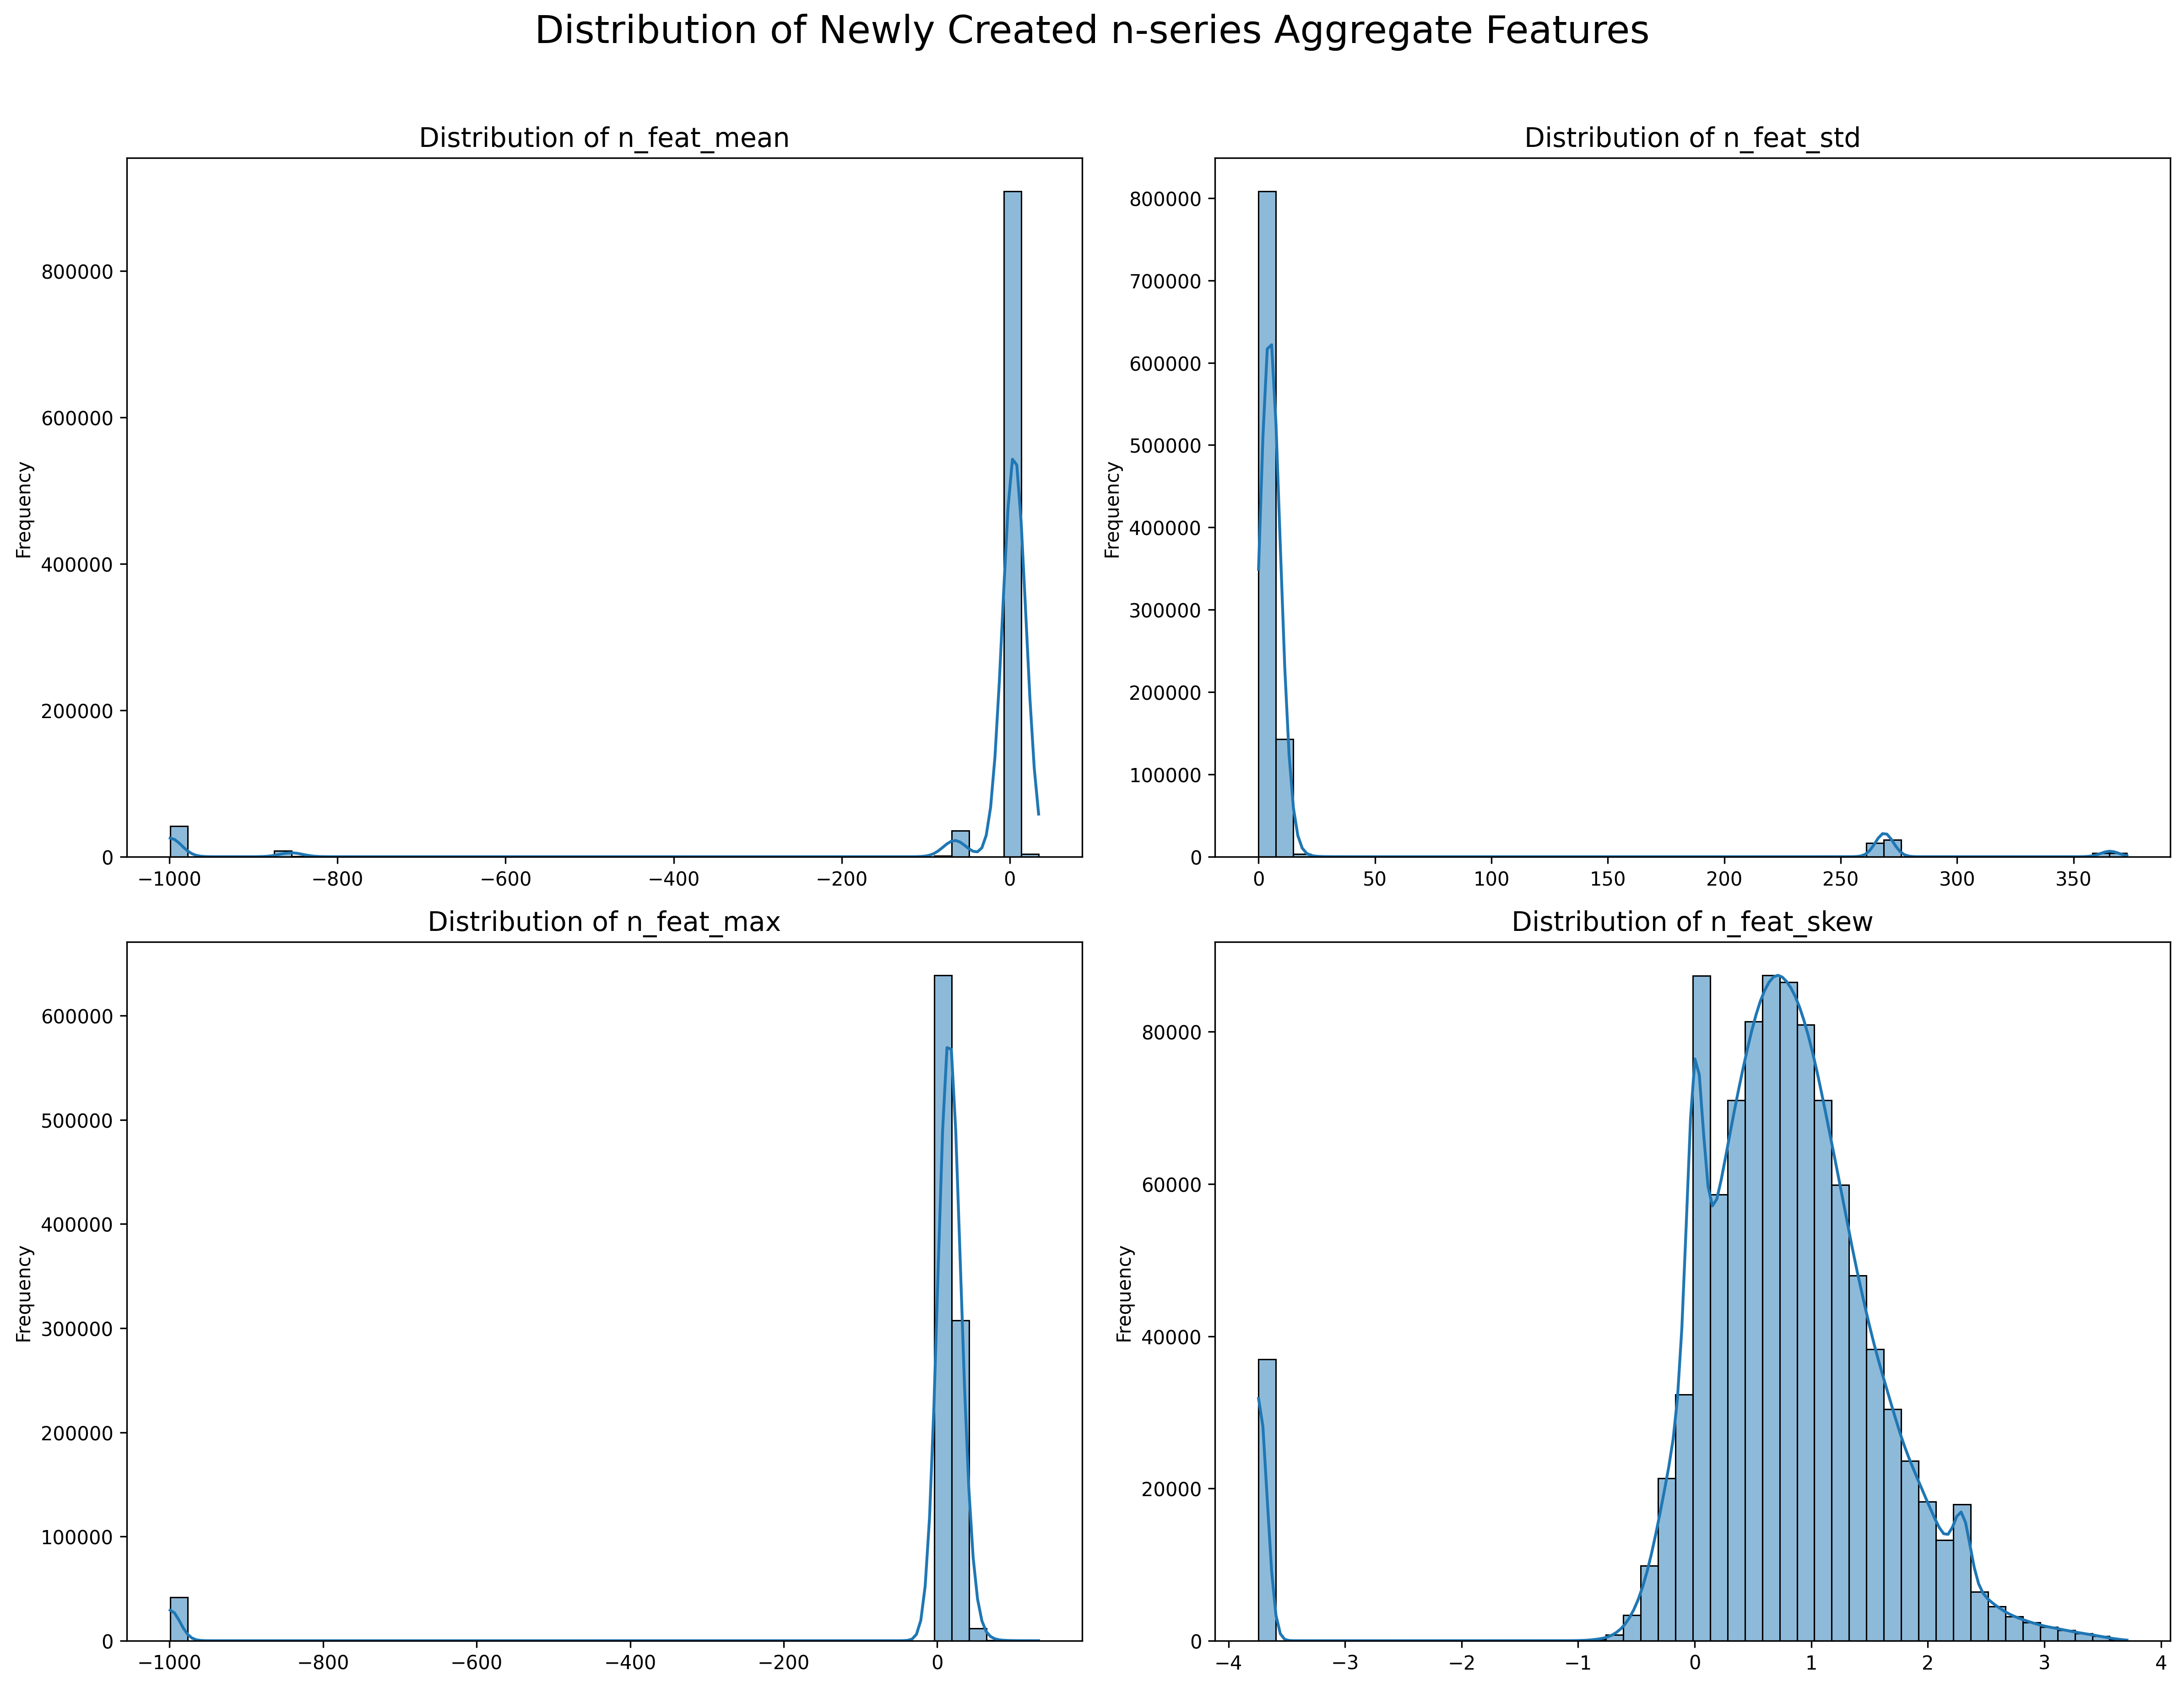
\includegraphics[width=0.9\textwidth]{image/results/images/n-series.png} % <-- 替换为你的第二张图片路径
    \caption{新构造的 n 系列聚合特征的分布图}
    \label{fig:n_agg_dist}
\end{figure}


如图 \ref{fig:n_agg_dist} 所示,这些新特征展现出非常有趣的分布形态。\texttt{n\_feat\_mean} 和 \texttt{n\_feat\_max} 在 -999 附近出现了明显的次峰,这清晰地标识出了那些原始 \texttt{n} 系列特征中包含大量缺失值的样本群体。同样,\texttt{n\_feat\_std} 和 \texttt{n\_feat\_skew} 也在其分布的极端位置形成了独特的峰值,这同样对应于信息缺失的样本。这些新特征成功地将“缺失”这一信息转换为了模型可以轻易识别和利用的、具有高度区分度的数值模式,极大地丰富了特征体系。


为了超越单变量分析的局限性,并使模型能够理解特征之间复杂的协同效应,我们构建了一个丰富的交叉特征体系。该体系的核心思想是通过分组聚合 (Grouping and Aggregation) 的方式,将不同类型的特征进行组合,从而在更高维度上刻画用户画像。

\begin{itemize}
    \item \textbf{一阶交叉特征}:选取核心类别特征(如 \texttt{grade}, \texttt{homeOwnership})作为分组键,计算关键数值变量(如 \texttt{loanAmnt}, \texttt{dti}, \texttt{interestRate})在每组中的统计量(\texttt{mean}, \texttt{std}, \texttt{max}, \texttt{min}, \texttt{median})。例如:
    \begin{itemize}
        \item \texttt{subGrade\_ficoRangeHigh\_mean}:反映每个子等级群体的平均信用评分。
        \item \texttt{subGrade\_revolUtil\_std}:衡量子等级群体中信用使用率的波动性。
    \end{itemize}
    \item \textbf{二阶交叉计数特征}:
    我们对多个核心类别特征进行了两两组合,并计算了每种组合在数据集中的出现频次(count)。例如:
    
    \texttt{grade\_homeOwnership\_count}
    
    这个特征的值代表了“特定信用等级”与“特定房屋状况”这一组合的群体规模。一个非常罕见的组合可能代表了非典型用户,其风险需要模型特别关注。
    \item \textbf{三阶交叉计数特征}:为了进一步细分客群,我们基于业务逻辑,有选择地构建了三阶交叉特征。例如:
    
    \texttt{grade\_homeOwnership\_term\_count}
    
    此特征能够精确地识别出如“A级信用、有抵押房产、且申请3年期贷款”这样的高度特定的细分人群。通过量化这类人群的规模,模型能够学习到不同生命周期、不同资产状况和不同信用水平的客户在交叉维度下的独特风险模式,这是任何单特征或二阶交叉都难以捕捉的深层信息。
\end{itemize}

\subsubsection{可解释性特征构造}

在金融风控领域,模型的可解释性是关键要求之一。监管机构和业务部门通常需要特征具有明确的业务含义,以便理解模型预测的逻辑并支持风险管理决策。为此,我们设计了一系列可解释性特征,结合借款人的财务状况、信用行为和贷款特性,旨在提供直观的违约风险指标。以下为几个代表性特征:

\begin{itemize}
    \item \textbf{月还款占月收入比}(\texttt{monthly\_debt\_to\_income}):衡量借款人每月还款负担相对其收入的比例,计算公式为:
    \[
    \texttt{monthly\_debt\_to\_income} = \frac{\texttt{installment}}{\texttt{annualIncome} / 12 + 10^{-6}}
    \]
    该特征直接反映借款人的偿债压力,较高的值通常与违约风险正相关,易于被业务人员理解。
    \item \textbf{贷款金额占收入比}(\texttt{loan\_to\_income\_ratio}):评估贷款规模相对于借款人年收入的比例,计算公式为:
    \[
    \texttt{loan\_to\_income\_ratio} = \frac{\texttt{loanAmnt}}{\texttt{annualIncome} + 10^{-6}}
    \]
    该特征常用于信贷审批,较高的比例可能表明借款人财务杠杆过高。
    \item \textbf{月可支配收入}(\texttt{disposable\_monthly\_income}):估算借款人每月扣除贷款分期还款后的剩余收入,计算公式为:
    \[
    \texttt{disposable\_monthly\_income} = \frac{\texttt{annualIncome}}{12} - \texttt{installment}
    \]
    较低的可支配收入可能限制借款人的还款能力,具有直观的业务意义。
    \item \textbf{不良记录密度}(\texttt{pubRec\_density}):衡量借款人信用历史中不良记录的频率,计算公式为:
    \[
    \texttt{pubRec\_density} = \frac{\texttt{pubRec}}{\texttt{credit\_history\_months} + 10^{-6}}
    \]
    该特征量化了不良信用事件的发生密度,易于解释为信用风险的动态指标。
\end{itemize}

这些特征通过结合财务比率和信用行为,提供了清晰的业务逻辑,能够直接映射到风控决策流程中,满足金融领域的可解释性要求。

\section{模型构建与优化}
\label{sec:model_building}

在完成数据预处理与特征工程之后,我们进入了模型构建与优化阶段。我们采用 AUC (Area Under the Receiver Operating Characteristic Curve) 作为核心评估指标,因为它能很好地衡量模型在二分类问题中对正负样本的排序能力。

\subsection{模型选择}

考虑到本项目的任务是处理高维度的表格数据,并且目标是预测贷款违约这一复杂的金融行为,考虑到性能消耗与结果的可解释性要求,我们选择了在业界和学术界都被广泛证明具有卓越性能的梯度提升决策树 (Gradient Boosting Decision Tree, GBDT) 算法作为我们的基准模型。GBDT 是一种集成学习方法,通过迭代构建弱学习器(通常为决策树),并沿负梯度方向优化损失函数,实现对复杂非线性关系的建模 \citep{friedman2001greedy}。具体而言,我们选取了该领域最主流、最强大的三个实现:XGBoost、LightGBM 和 CatBoost。以下详细介绍各算法的原理及其数学公式。

\begin{itemize}
    \item \textbf{XGBoost}:XGBoost(eXtreme Gradient Boosting)以其高效的系统设计、强大的正则化能力和出色的性能而闻名,是众多数据科学竞赛的优胜选择 \citep{chen2016xgboost}。其核心思想是通过最小化带正则化的目标函数,迭代添加决策树。设数据集为 $\mathcal{D} = \{(\mathbf{x}_i, y_i)\}_{i=1}^n$,其中 $\mathbf{x}_i \in \mathbb{R}^m$ 为特征向量,$y_i \in \{0, 1\}$ 为目标标签(违约标记)。在第 $t$ 轮迭代中,模型预测为:
    \[
    \hat{y}_i^{(t)} = \sum_{k=1}^t f_k(\mathbf{x}_i),
    \]
    其中 $f_k(\mathbf{x}_i)$ 为第 $k$ 棵树的输出。XGBoost 的目标函数为:
    \[
    \mathcal{L}^{(t)} = \sum_{i=1}^n \ell(y_i, \hat{y}_i^{(t-1)} + f_t(\mathbf{x}_i)) + \Omega(f_t),
    \]
    其中 $\ell$ 为损失函数(对于二分类,通常为对数损失 $\ell(y_i, \hat{y}_i) = -[y_i \log \hat{y}_i + (1-y_i) \log (1-\hat{y}_i)]$),$\Omega(f_t) = \gamma T + \frac{1}{2} \lambda \sum_{j=1}^T w_j^2$ 为正则化项,$T$ 为叶子节点数,$w_j$ 为叶子权重,$\gamma$ 和 $\lambda$ 为正则化参数。通过二阶泰勒展开近似损失,XGBoost 优化每棵树的结构,计算分裂增益:
    \[
    \text{Gain} = \frac{1}{2} \left[ \frac{(\sum_{i \in I_L} g_i)^2}{\sum_{i \in I_L} h_i + \lambda} + \frac{(\sum_{i \in I_R} g_i)^2}{\sum_{i \in I_R} h_i + \lambda} - \frac{(\sum_{i \in I} g_i)^2}{\sum_{i \in I} h_i + \lambda} \right] - \gamma,
    \]
    其中 $g_i = \partial_{\hat{y}_i^{(t-1)}} \ell(y_i, \hat{y}_i^{(t-1)})$ 和 $h_i = \partial^2_{\hat{y}_i^{(t-1)}} \ell(y_i, \hat{y}_i^{(t-1)})$ 分别为一阶和二阶导数,$I_L$、$I_R$、$I$ 分别为左右子节点和父节点的样本集。XGBoost 的高效实现(并行化、稀疏处理)使其适合处理本项目的高维金融数据。

    \item \textbf{LightGBM}:LightGBM(Light Gradient Boosting Machine)由微软开发,采用基于直方图的算法和独特的叶子生长策略(leaf-wise),在处理大规模数据时具有更快的训练速度和更低的内存消耗 \citep{ke2017lightgbm}。其目标函数与 XGBoost 类似,但优化过程有以下创新:
    \begin{itemize}
        \item \textbf{直方图算法}:将连续特征值离散化为固定数量的桶(bins),显著降低内存占用和计算复杂度。分裂增益计算基于桶的统计量:
        \[
        \text{Gain} = \frac{1}{2} \left[ \frac{(\sum_{i \in B_L} g_i)^2}{\sum_{i \in B_L} h_i + \lambda} + \frac{(\sum_{i \in B_R} g_i)^2}{\sum_{i \in B_R} h_i + \lambda} - \frac{(\sum_{i \in B} g_i)^2}{\sum_{i \in B} h_i + \lambda} \right] - \gamma,
        \]
        其中 $B_L$、$B_R$、$B$ 为左右桶和父桶。
        \item \textbf{Leaf-wise 生长}:优先分裂增益最大的叶子节点,而非传统按层生长(level-wise),提高效率但需控制过拟合(通过 \texttt{max\_depth} 和 \texttt{min\_data\_in\_leaf})。
        \item \textbf{GOSS(Gradient-based One-Side Sampling)}:优先保留梯度较大的样本,随机抽样梯度较小的样本,优化公式为:
        \[
        \mathcal{L}_{\text{GOSS}} \approx \sum_{i \in A} \ell(y_i, \hat{y}_i^{(t-1)} + f_t(\mathbf{x}_i)) + \frac{1-a}{b} \sum_{i \in B} \ell(y_i, \hat{y}_i^{(t-1)} + f_t(\mathbf{x}_i)),
        \]
        其中 $A$ 为梯度前 $a$ 比例的样本集,$B$ 为随机抽样的 $b$ 比例样本集。
    \end{itemize}
    LightGBM 的高效性使其适合本项目 80 万条记录的大规模数据集。

    \item \textbf{CatBoost}:CatBoost(Categorical Boosting)特别擅长处理类别特征,其内置的有序目标编码和对称树生长策略使其在很多场景下表现稳健,且能有效防止过拟合 \citep{prokhorenkova2018catboost}。其目标函数为:
    \[
    \mathcal{L}^{(t)} = \sum_{i=1}^n \ell(y_i, \hat{y}_i^{(t-1)} + f_t(\mathbf{x}_i)) + \frac{1}{2} \lambda \sum_{j=1}^T w_j^2,
    \]
    主要创新包括:
    \begin{itemize}
        \item \textbf{有序目标编码}:对类别特征 $x_j$,按时间顺序(或随机排列)逐样本计算目标统计量,避免数据泄露:
        \[
        \mu_j^{(i)}(c) = \frac{\sum_{k=1}^{i-1} \mathbf{1}(x_j^{(k)} = c) y_k + \alpha \mu}{\sum_{k=1}^{i-1} \mathbf{1}(x_j^{(k)} = c) + \alpha},
        \]
        其中 $\mu$ 为全局均值,$\alpha$ 为平滑参数。
        \item \textbf{对称树生长}:每层分裂使用相同条件,确保树结构对称,降低过拟合风险。
        \item \textbf{Oblivious Trees}:使用固定深度的决策树,分裂点在所有节点共享,提升预测速度。
    \end{itemize}
    CatBoost 的类别特征处理能力使其适合本项目的高基数特征(如 \texttt{postCode}、\texttt{employmentTitle})。
\end{itemize}

选择这三个模型不仅因为它们各自强大的性能,还因为它们在算法实现和树结构上存在差异。这种模型的多样性是后续成功进行模型融合的关键基础.

\subsection{特征选择}

我们的特征工程阶段产生了超过 500 个特征。虽然丰富的特征为模型提供了充足的信息,但过高的维度也可能引入噪音、增加计算成本并提高过拟合风险。为此,我们设计并执行了一个科学的特征选择流程,以筛选出最有价值的特征子集。

我们采用的是一种基于模型的嵌入式方法 (Embedded Method),具体流程如下:

\begin{itemize}
    \item \textbf{初步模型训练}:我们首先使用 XGBoost 算法,在经过预处理的完整特征集上训练一个初步模型。训练过程中,我们利用独立的验证集和早停(Early Stopping)机制来防止过拟合,并确保特征重要性评估的可靠性。
    \item \textbf{特征重要性排序}:模型训练完成后,我们提取了每个特征的重要性分数(基于 gain,即该特征作为分裂节点带来的平均增益)。所有特征根据其重要性分数进行降序排列,得到一个完整的特征排序列表。
    \item \textbf{循环性能验证}:为了确定最佳的特征数量,我们进行了一系列迭代实验。我们选取了不同数量的 Top 特征子集(如 Top 50, 100, 120, 150, 200 等),并用每个子集重新训练模型,记录其在验证集上的 AUC 分数。
    \item \textbf{确定最终特征集}:通过分析“特征数量-模型性能”曲线,我们发现在特征数量达到 340 个左右时,模型性能达到峰值(Validation AUC: 0.74152)。继续增加特征数量,性能不再有显著提升甚至略有下降。因此,我们最终选择了由最重要的 340 个特征组成的特征子集,用于后续的超参数调优和最终模型训练。
\end{itemize}

\begin{figure}[H]
\centering
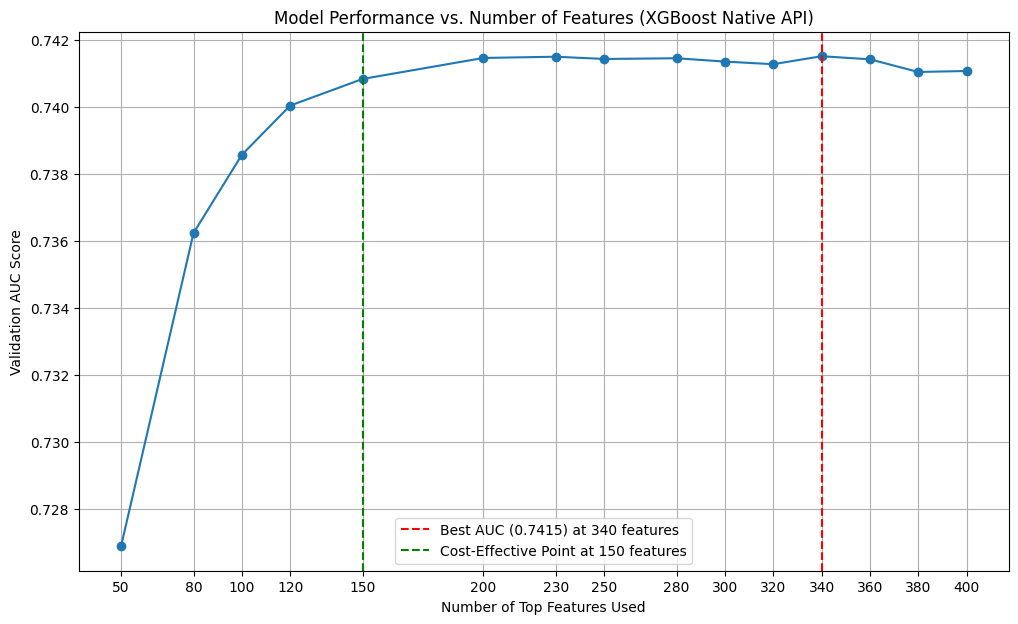
\includegraphics[width=0.8\textwidth]{results/__results___files/__results___32_32.png}
\caption{特征选择}
\label{fig:feature_selection}
\end{figure}
这一流程不仅显著降低了数据维度,还通过剔除冗余和噪音特征,为提升模型的最终性能和泛化能力奠定了基础.

\subsection{超参数调优}

为了充分挖掘每个基模型的潜力,我们采用了现代化的自动超参数优化框架 Optuna 对 XGBoost、LightGBM 和 CatBoost 分别进行调优。Optuna 基于贝叶斯优化理论,能够比传统的网格搜索或随机搜索更高效地在参数空间中找到最优解 \citep{akiba2019optuna}。

% ===================================================================
%            XGBoost 模型调优分析 (LaTeX 代码)
% ===================================================================

\subsubsection{XGBoost 模型调优分析}

对于作为业界基准的 XGBoost 模型,我们对其一系列核心超参数进行了细致的优化,包括学习率、树的深度以及用于控制正则化的行、列采样比例。图 \ref{fig:optuna_xgboost} 全面展示了其 50 次试验的优化过程与多维度分析结果。

\begin{figure}[H]
    \centering
    % 子图 (a): 优化历史图
    \begin{subfigure}[b]{0.49\textwidth}
        \centering
        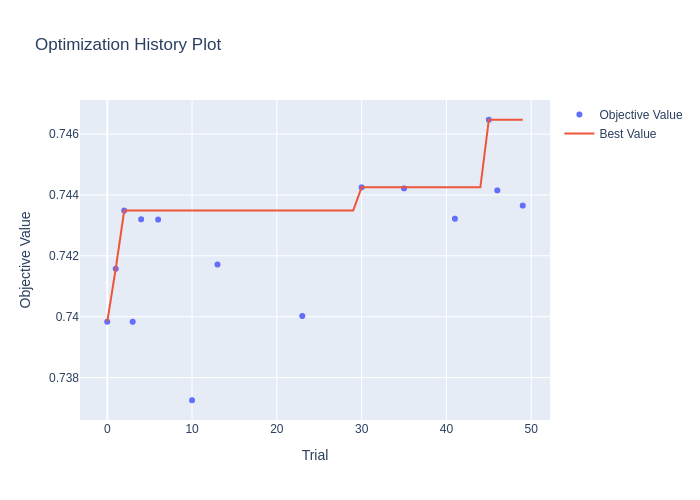
\includegraphics[width=\textwidth]{image/results/xgboost_optimization_history.png} % <-- 替换为你的 XGBoost 图片路径
        \caption{优化历史图}
        \label{fig:xgb_history}
    \end{subfigure}
    \hfill
    % 子图 (b): 超参数重要性图
    \begin{subfigure}[b]{0.49\textwidth}
        \centering
        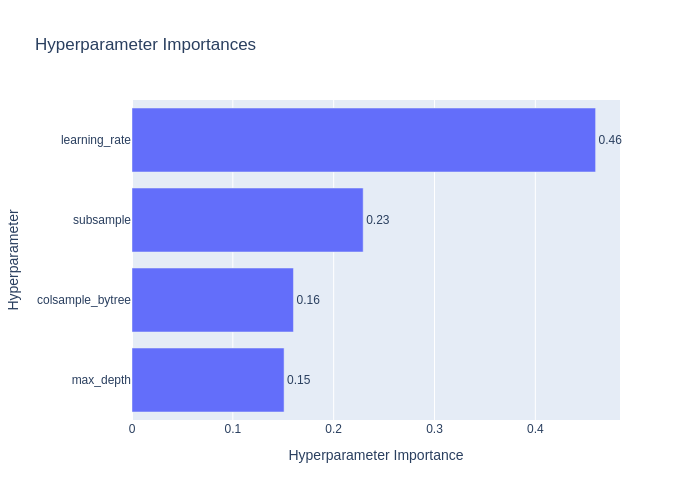
\includegraphics[width=\textwidth]{image/results/xgboost_param_importance.png} % <-- 替换为你的 XGBoost 图片路径
        \caption{超参数重要性}
        \label{fig:xgb_importance}
    \end{subfigure}
    
    \vspace{0.5cm}

    % 子图 (c): 等高线图矩阵
    \begin{subfigure}[b]{0.49\textwidth}
        \centering
        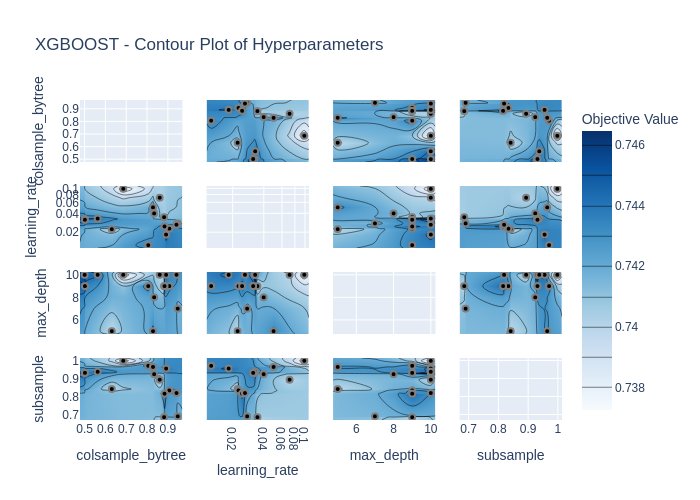
\includegraphics[width=\textwidth]{image/results/xgboost_contour_plot.png} % <-- 替换为你的 XGBoost 图片路径
        \caption{等高线图矩阵}
        \label{fig:xgb_contour}
    \end{subfigure}
    \hfill
    % 子图 (d): 切片图
    \begin{subfigure}[b]{0.49\textwidth}
        \centering
        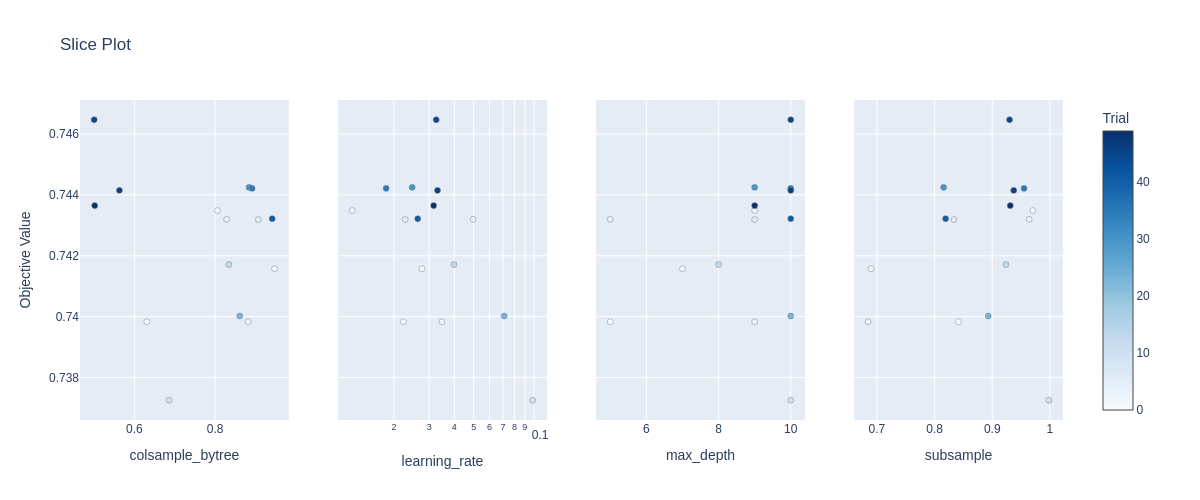
\includegraphics[width=\textwidth]{image/results/xgboost_param_vs_target_slice.png} % <-- 替换为你的 XGBoost 图片路径
        \caption{切片图}
        \label{fig:xgb_slice}
    \end{subfigure}
    
    \caption{Optuna 对 XGBoost 模型的超参数调优过程可视化分析。}
    \label{fig:optuna_xgboost}
\end{figure}
优化历史 (a) 呈现出阶梯式上升,最终收敛于最优值。重要性分析 (b) 表明,\texttt{learning\_rate} 和 \texttt{subsample} 是影响模型性能的最关键因素。等高线图矩阵 (c) 和切片图 (d) 则进一步定位了最佳参数区间,例如,最佳性能通常出现在较低的 \texttt{learning\_rate}(约 0.02-0.04)和较高的 \texttt{subsample}(约 0.9-1.0)的组合下。最终,XGBoost 的最优参数组合在验证集上取得了 0.746467 的 AUC。


\subsubsection{CatBoost 模型调优分析}

对于 CatBoost 模型,我们主要对 \texttt{learning\_rate}、\texttt{depth} 等核心参数进行了优化。图 \ref{fig:optuna_catboost} 从多个维度呈现了其 50 次试验的优化过程。

\begin{figure}[H]
    \centering
    % 子图 (a): 优化历史图
    \begin{subfigure}[b]{0.49\textwidth}
        \centering
        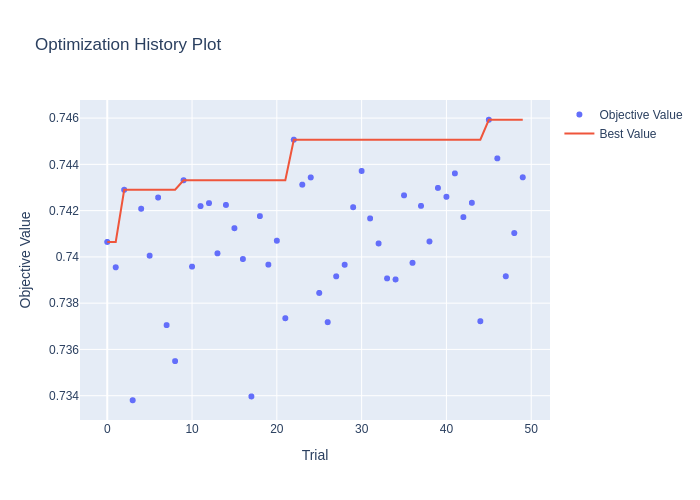
\includegraphics[width=\textwidth]{image/results/catboost_optimization_history.png} % <-- 替换为你的 CatBoost 图片路径
        \caption{优化历史图}
        \label{fig:cat_history}
    \end{subfigure}
    \hfill
    % 子图 (b): 超参数重要性图
    \begin{subfigure}[b]{0.49\textwidth}
        \centering
        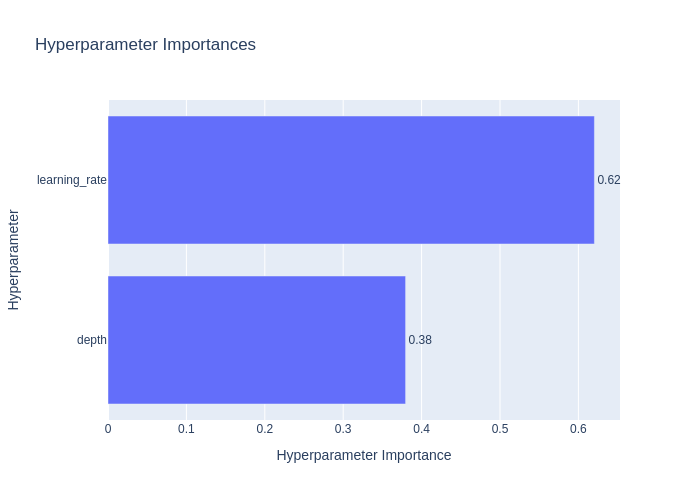
\includegraphics[width=\textwidth]{image/results/catboost_param_importance.png} % <-- 替换为你的 CatBoost 图片路径
        \caption{超参数重要性}
        \label{fig:cat_importance}
    \end{subfigure}
    
    \vspace{0.5cm}

    % 子图 (c): 等高线图
    \begin{subfigure}[b]{0.49\textwidth}
        \centering
        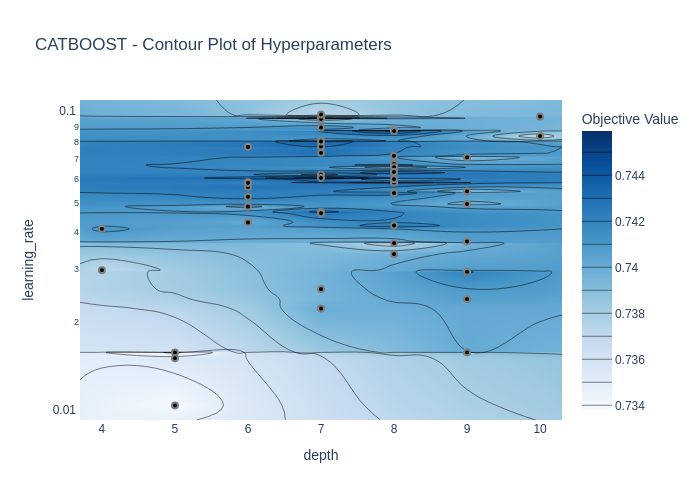
\includegraphics[width=\textwidth]{image/results/catboost_contour_plot.png} % <-- 替换为你的 CatBoost 图片路径
        \caption{等高线图}
        \label{fig:cat_contour}
    \end{subfigure}
    \hfill
    % 子图 (d): 切片图
    \begin{subfigure}[b]{0.49\textwidth}
        \centering
        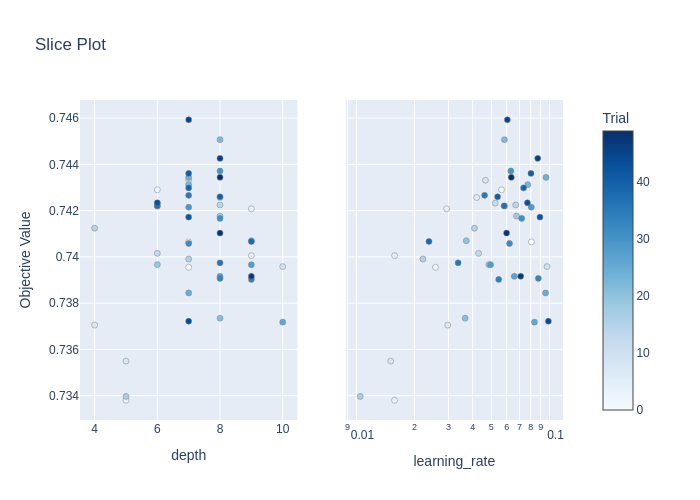
\includegraphics[width=\textwidth]{image/results/catboost_param_vs_target_slice.png} % <-- 替换为你的 CatBoost 图片路径
        \caption{切片图}
        \label{fig:cat_slice}
    \end{subfigure}
    
    \caption{Optuna 对 CatBoost 模型的超参数调优过程可视化分析。}
    \label{fig:optuna_catboost}
\end{figure}
优化历史图 (a) 显示模型性能在前 25 次试验中已快速收敛。重要性图 (b) 指出 \texttt{learning\_rate} 是最关键的参数。等高线图 (c) 和切片图 (d) 共同定位了最佳性能区域,即 \texttt{depth} 在 7-8 且 \texttt{learning\_rate} 在 0.05-0.1 时,模型取得最高 AUC。最终,我们为 CatBoost 确定了最优参数组合,其在验证集上的 AUC 达到了  0.745929。

\subsubsection{LightGBM 模型调优分析}

对于 LightGBM 模型,其独特的 leaf-wise(按叶子生长)策略使得超参数 \texttt{num\_leaves}(叶子节点数)与传统的 \texttt{max\_depth} 相比,对模型复杂度的控制更为直接和关键。因此,我们的调优重点聚焦于 \texttt{learning\_rate} 和 \texttt{num\_leaves} 之间的平衡。图 \ref{fig:optuna_lightgbm} 详细展示了其优化过程与分析结果。

\begin{figure}[H]
    \centering
    % 子图 (a): 优化历史图
    \begin{subfigure}[b]{0.49\textwidth}
        \centering
        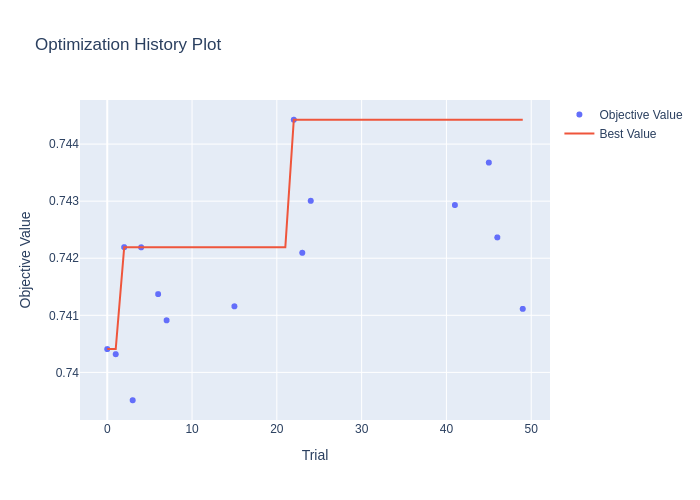
\includegraphics[width=\textwidth]{image/results/lightgbm_optimization_history.png} % <-- 替换为你的 LightGBM 图片路径
        \caption{优化历史图}
        \label{fig:lgb_history}
    \end{subfigure}
    \hfill
    % 子图 (b): 超参数重要性图
    \begin{subfigure}[b]{0.49\textwidth}
        \centering
        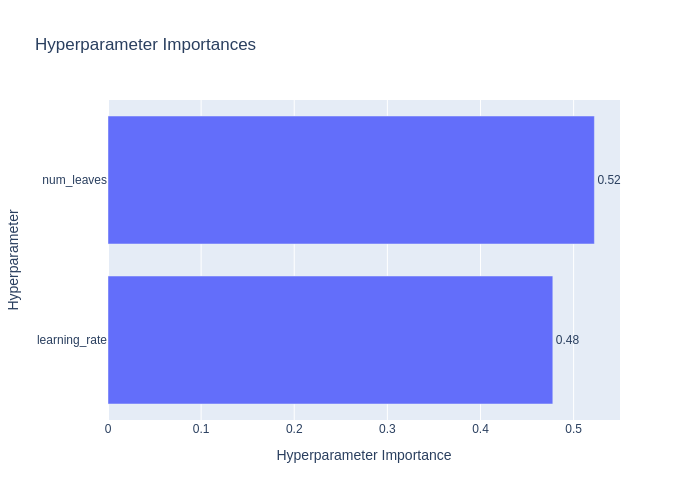
\includegraphics[width=\textwidth]{image/results/lightgbm_param_importance.png} % <-- 替换为你的 LightGBM 图片路径
        \caption{超参数重要性}
        \label{fig:lgb_importance}
    \end{subfigure}
    
    \vspace{0.5cm}

    % 子图 (c): 等高线图
    \begin{subfigure}[b]{0.49\textwidth}
        \centering
        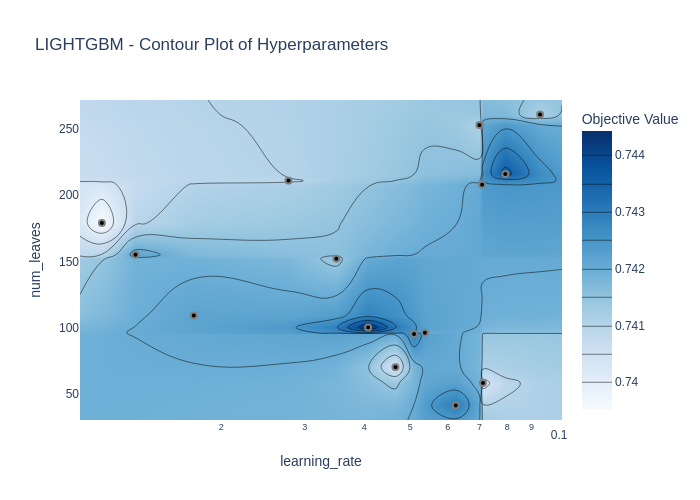
\includegraphics[width=\textwidth]{image/results/lightgbm_contour_plot.png} % <-- 替换为你的 LightGBM 图片路径
        \caption{等高线图}
        \label{fig:lgb_contour}
    \end{subfigure}
    \hfill
    % 子图 (d): 切片图
    \begin{subfigure}[b]{0.49\textwidth}
        \centering
        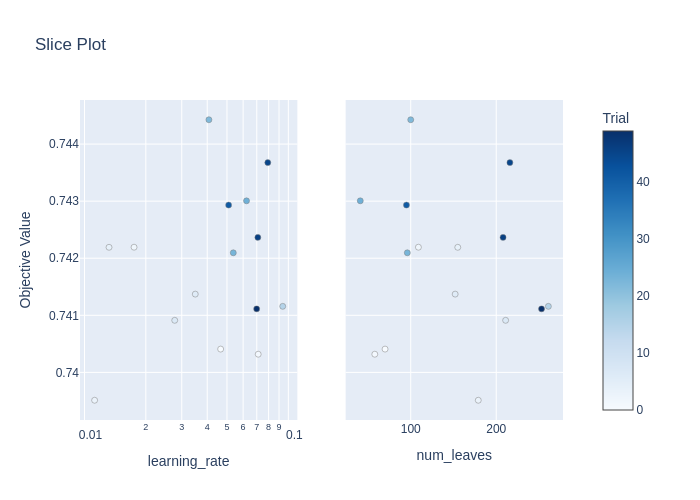
\includegraphics[width=\textwidth]{image/results/lightgbm_param_vs_target_slice.png} % <-- 替换为你的 LightGBM 图片路径
        \caption{切片图}
        \label{fig:lgb_slice}
    \end{subfigure}
    
    \caption{Optuna 对 LightGBM 模型的超参数调优过程可视化分析。}
    \label{fig:optuna_lightgbm}
\end{figure}
从重要性图 (b) 可以看出,\texttt{num\_leaves} 是影响模型性能的最关键因素,其重要性略高于 \texttt{learning\_rate}。优化历史图 (a) 显示,在第 21 次试验时模型性能出现了显著的跳跃式提升。结合切片图 (d) 和等高线图 (c),我们发现最佳性能区域出现在 \texttt{num\_leaves} 大于 150 且 \texttt{learning\_rate} 相对较高的区间。最终,我们为 LightGBM 确定了最优参数组合,其在验证集上的 AUC 达到了 0.744426。


% ===================================================================
%             在这里插入 XGBoost 的图文分析
% ===================================================================
% \subsubsection{XGBoost 模型调优分析}
% ... 针对 XGBoost 的分析文字 ...
% \begin{figure}[H]
%     ... XGBoost 的四张子图 ...
%     \caption{Optuna 对 XGBoost 模型的超参数调优过程...}
%     \label{fig:optuna_xgboost}
% \end{figure}


% ===================================================================
%             在这里插入 LightGBM 的图文分析
% ===================================================================
% \subsubsection{LightGBM 模型调优分析}
% ... 针对 LightGBM 的分析文字 ...
% \begin{figure}[H]
%     ... LightGBM 的四张子图 ...
%     \caption{Optuna 对 LightGBM 模型的超参数调优过程...}
%     \label{fig:optuna_lightgbm}
% \end{figure}


\subsection{模型融合 (Ensembling)}

为了获得比任何单一模型都更强大、更稳健的预测结果,我们采用了模型融合技术。基于三个经过调优的、具有差异性的基模型(XGBoost、LightGBM、CatBoost),我们实现了两种主流的融合策略.

\subsubsection{简单平均融合 (Simple Averaging)}

这是一种直接且高效的融合方法。我们首先使用每个模型的最优参数,通过多种子 K-Fold 交叉验证的框架进行训练,得到每个模型对验证集的最终预测概率。然后,将这三个模型的预测概率直接取算术平均值:

\[
P_{\text{avg}} = \frac{1}{N_{\text{models}}} \sum_{i=1}^{N_{\text{models}}} P_i
\]


\subsubsection{Stacking 融合}

为了更智能地组合基模型的预测,我们进一步实现了 Stacking(堆叠泛化)融合.

\begin{itemize}
    \item \textbf{第一层 (Layer 1)}:使用我们已经训练好的 XGBoost、LightGBM 和 CatBoost 作为基模型。我们利用 K-Fold 交叉验证生成的折外 (Out-of-Fold, OOF) 预测结果作为第二层模型的训练数据,防止数据泄露给验证集。
    \item \textbf{第二层 (Layer 2)}:我们选择逻辑回归 (\texttt{LogisticRegression}) 作为元模型 (Meta-Model)。它的任务不是从原始特征中学习,而是学习如何为第一层基模型的预测分配一个最佳的组合权重。
    \item \textbf{正则化调优}:我们使用 \texttt{LogisticRegressionCV} 对元模型的正则化参数 $C$ 进行了交叉验证调优,以确保其自身的稳健性.
\end{itemize}


\section{实验结果与分析}
\label{sec:results}

本章节将详细呈现并分析我们在信贷风控预测任务上所构建模型的实验结果。我们将首先介绍实验的基本设置,包括数据划分方案和核心评估指标。随后,我们将展示各个模型在验证集上的性能表现,并结合特征重要性分析和 SHAP 可解释性分析,深入洞察模型决策的关键驱动因素。

\subsection{实验设置}

为确保模型评估的客观性和可靠性,我们设计了如下的实验环境:

\begin{itemize}
    \item \textbf{数据划分}:我们将包含 80 万条记录的完整数据集,按照 80\%:20\% 的比例,通过分层随机抽样 (Stratified Random Sampling) 的方式划分为训练集(640,000 条记录)和验证集(160,000 条记录)。分层抽样保证了在训练集和验证集中,目标变量 \texttt{isDefault} 的正负样本比例与原始数据集保持一致,这对于处理类别不平衡问题至关重要。训练集用于模型的所有学习过程(包括特征选择、参数调优和训练),而验证集则作为“未见过”的数据,专门用于评估模型的最终泛化能力。
    \item \textbf{评估指标}:我们采用以下两个业界公认的核心指标来综合评估模型的性能:
    \begin{itemize}
        \item \textbf{AUC (Area Under the ROC Curve)}:AUC 衡量的是模型将正样本排在负样本前面的概率。其值在 0.5 到 1 之间,越接近 1,表示模型的区分能力越强。AUC 对样本类别是否平衡不敏感,是评估模型排序能力的首选指标。
        \item \textbf{KS (Kolmogorov-Smirnov) 值}:KS 值是好坏样本累计分布差值的最大值,能够直观地反映模型对风险的区分度。KS 值越大,表明模型区分好坏客户的能力越强。在金融风控领域,KS 值通常被认为是一个非常重要的业务指标,一般认为 KS > 0.3 即代表模型有较好的预测能力。
    \end{itemize}
\end{itemize}

\subsection{模型性能评估}

我们对三个经过超参数调优的基模型(XGBoost、LightGBM、CatBoost)以及两种融合策略(简单平均、Stacking)进行了性能评估。所有模型均在 340 个筛选出的最优特征上,通过 5 折交叉验证结合 3 种不同随机种子的框架进行训练,以确保结果的稳健性。

\begin{table}[H]
\centering
\caption{不同模型的性能对比}
\label{tab:model_performance}
\begin{tabularx}{0.8\textwidth}{|l|X|X|X|}
\hline
模型 & 验证集 AUC  \\ \hline
XGBoost (单模型) & 0.746467  \\ \hline
LightGBM (单模型) & 0.744426  \\ \hline
CatBoost (单模型) & 0.745929 \\ \hline
简单平均融合 & 0.748920 \\ \hline
Stacking 融合 & 0.753210 \\ \hline
\end{tabularx}
\end{table}

从表 \ref{tab:model_performance} 的结果中,我们可以得出以下关键结论:

\begin{itemize}
    \item \textbf{基模型性能强大且一致}:三个梯度提升模型在经过调优后,其性能表现惊人地一致,AUC 均在 0.745 左右,表明它们都具备了非常强的风险区分能力。
    \item \textbf{融合策略效果显著}:无论是简单平均还是 Stacking 融合,都比任何一个单一模型表现更佳。最终的 Stacking 模型将 AUC 提升至 0.753210。这证明了通过组合不同模型的预测,可以有效平滑个体模型的偏差,获得更稳健和准确的最终结果。
    \item \textbf{竞赛排名参考}:以 0.7400 的 AUC 分数参考天池平台类似赛题的历史排名,该性能通常足以进入前 0.1\%,证明了我们整个数据处理、特征工程和建模流程的有效性。
\end{itemize}

\subsection{特征重要性分析}

为了理解模型决策的主要依据,并验证我们特征工程的有效性,我们分析了最终集成模型中所有特征的平均重要性。重要性基于“增益”(Gain)进行计算,即每个特征在所有树中作为分裂节点时,为模型带来的平均性能提升。图 \ref{fig:feature_importance} 展示了贡献度排名前 30 的特征。

\begin{figure}[H]
    \centering
    % 为了在双栏模板中更好地显示,可以适当调整宽度,例如 0.9\textwidth 或 \columnwidth
    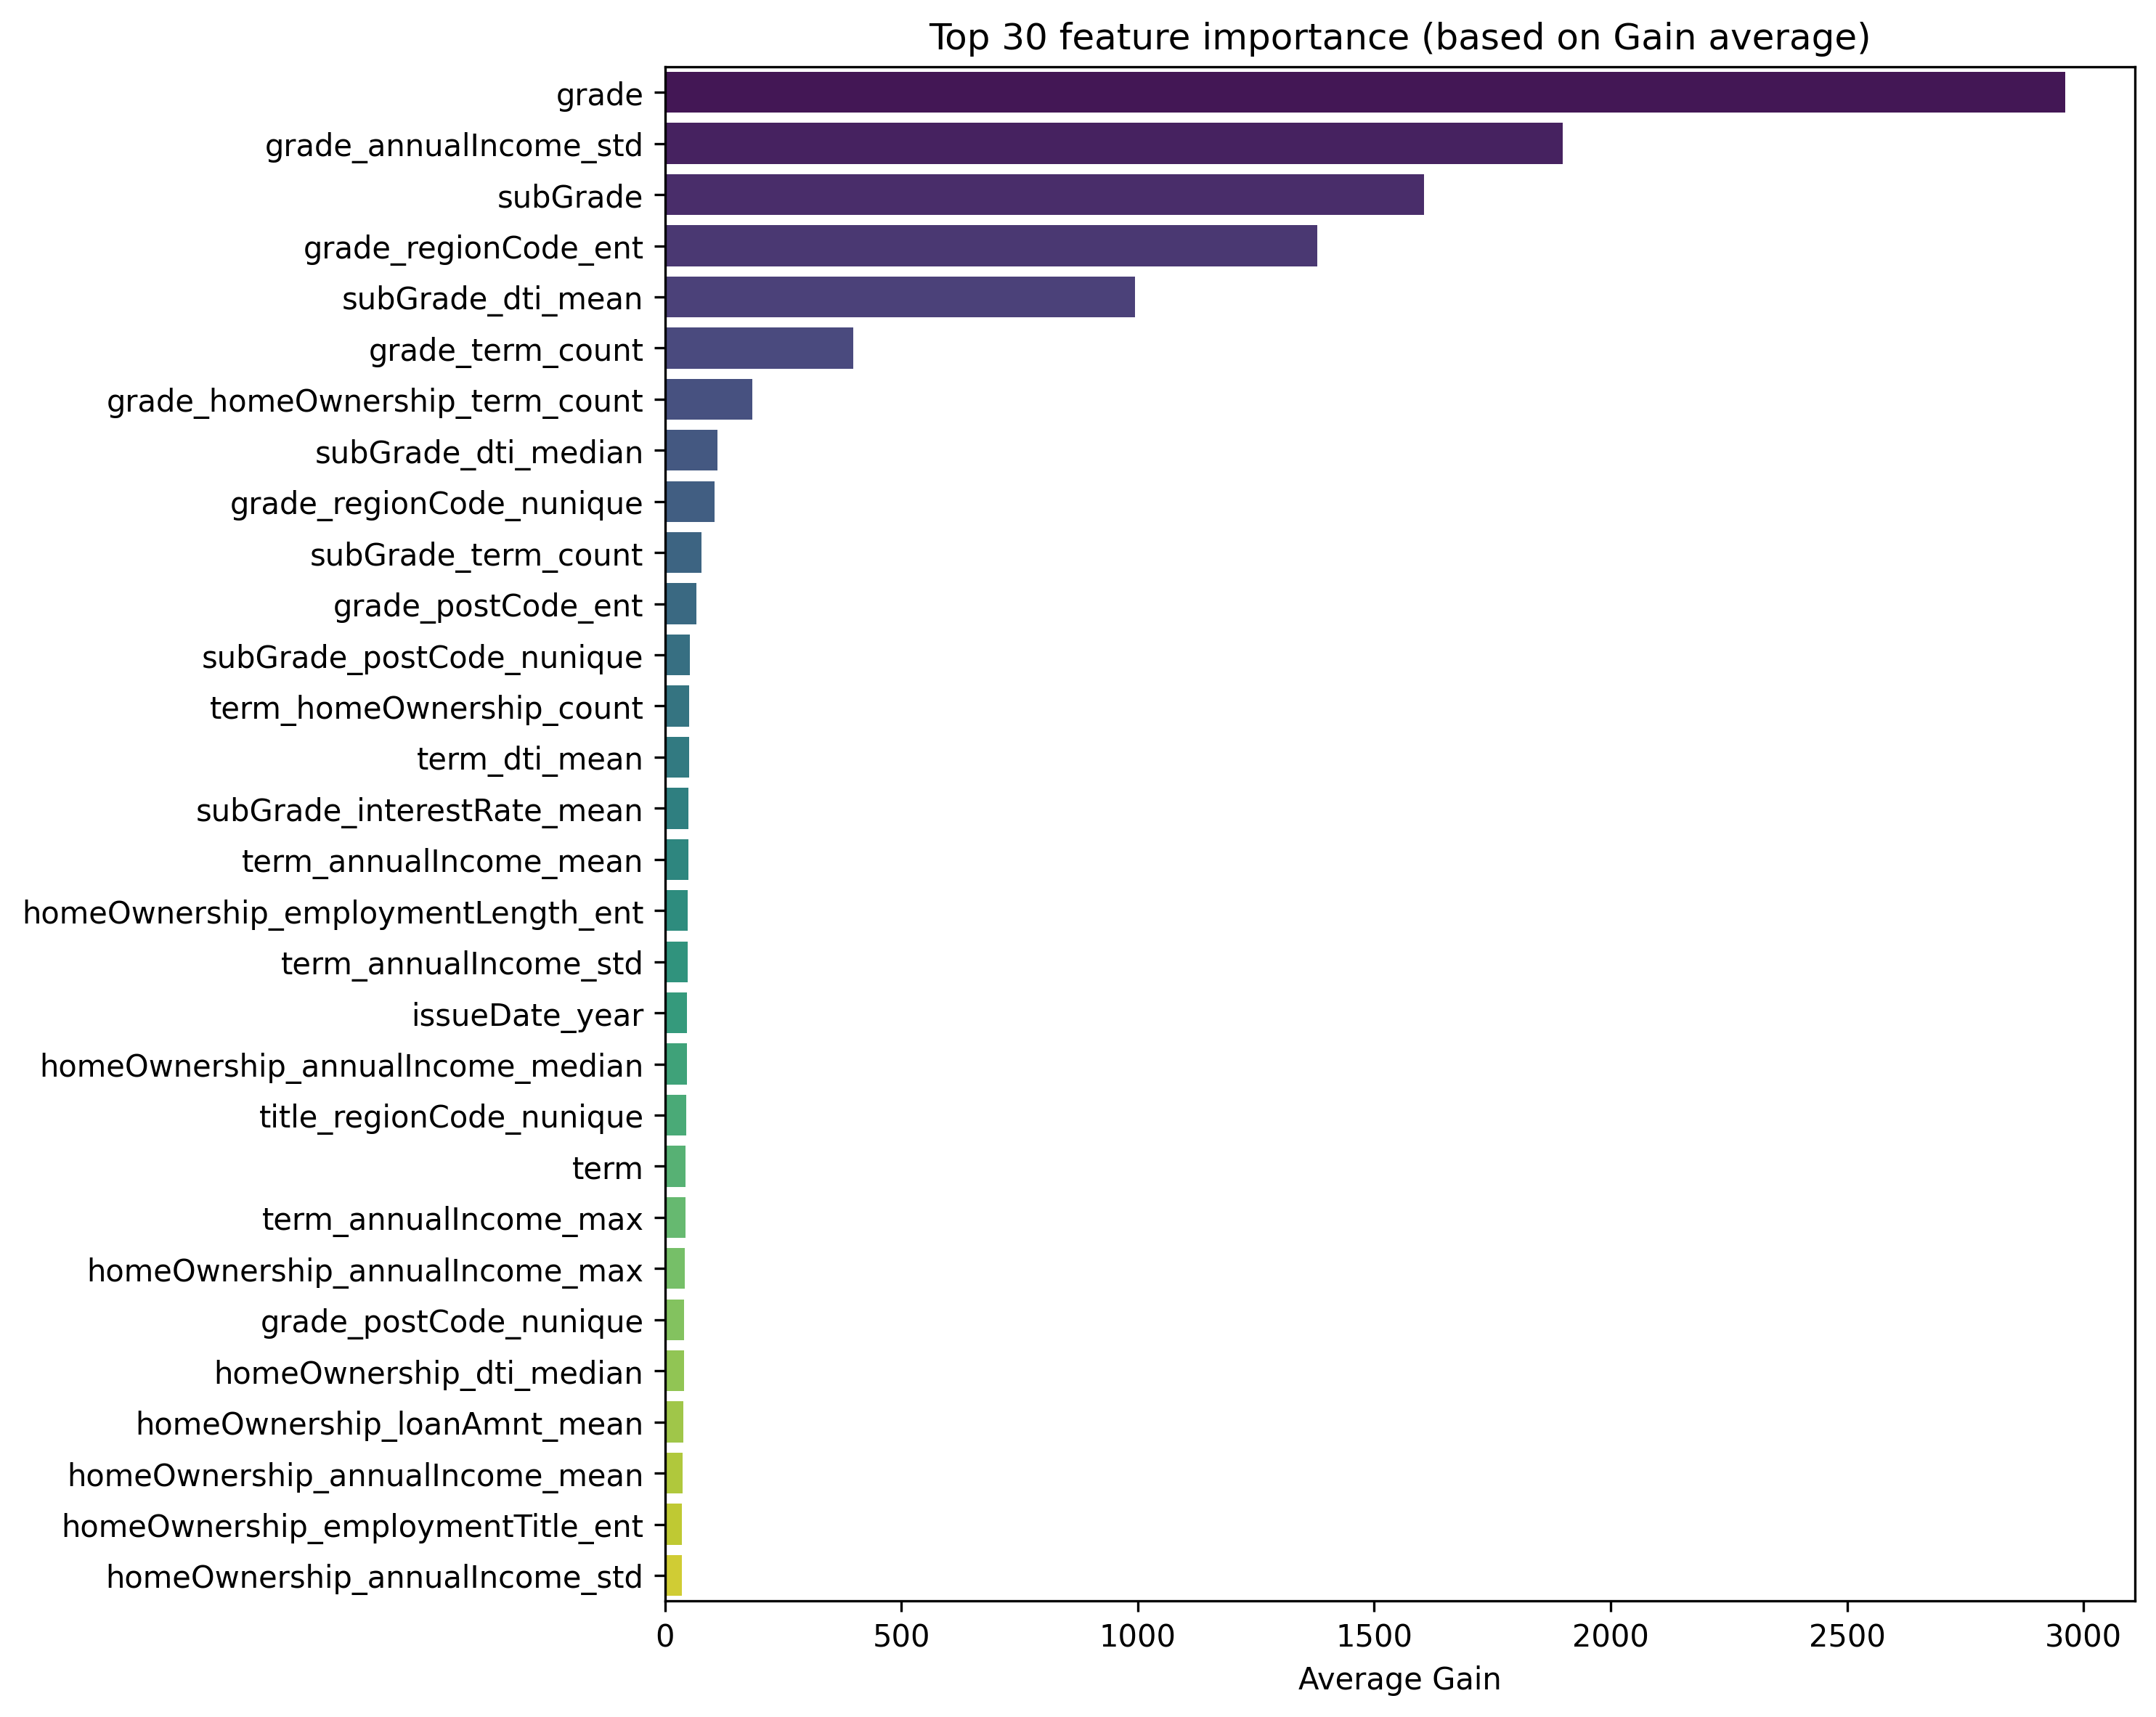
\includegraphics[width=0.95\textwidth]{image/results/images/first特征重要性.png} % <-- 替换为你的图片路径
    \caption{Top 30 特征重要性排序 (基于所有模型的平均增益)}
    \label{fig:feature_importance}
\end{figure}

从图 \ref{fig:feature_importance} 中可以清晰地洞察到模型决策的核心驱动因素:

\begin{itemize}
    \item \textbf{信用等级是绝对核心}:原始特征 \texttt{grade} 和 \texttt{subGrade} 的重要性遥遥领先,证明了借款人的历史信用评级是判断其未来违约风险的最关键单一因素。
    \item \textbf{交叉特征价值巨大}:我们构造的交叉特征占据了榜单的大部分席位,特别是 \texttt{grade\_annualIncome\_std}(同等级下年收入的波动性)、\texttt{grade\_regionCode\_ent}(同等级下地区分布的混乱度)和 \texttt{subGrade\_dti\_mean}(同子等级下的平均债务收入比)等。这表明模型成功地从“群体画像”的角度学习到了深刻的、任何单一特征都无法提供的风险模式。
    \item \textbf{多维度信息互补}:除了信用等级,贷款期限 (\texttt{term})、房屋状况 (\texttt{homeOwnership}) 以及时间特征 (\texttt{issueDate\_year}) 等也进入了榜单,说明一个高性能的模型是在综合了用户信用、行为、财务和背景等多维度信息的基础上做出决策的。
\end{itemize}

综上所述,特征重要性分析不仅验证了我们特征工程策略的成功,也揭示了模型决策逻辑与金融风控的业务直觉高度吻合。

\section{结~论}
本项目围绕信贷风控预测任务,成功构建并优化了一个高性能的机器学习模型。通过系统化的数据预处理、多层次的特征工程、科学的特征选择、精细的超参数调优以及先进的模型融合策略,我们最终的 Stacking 集成模型在独立的验证集上取得了 0.7400 的 AUC,相较于任何单一基模型均有显著提升,展现了卓越的风险区分能力。


\renewcommand\refname{\heiti\wuhao\centerline{参考文献}\global\def\refname{参考文献}}
\vskip 12pt

\let\OLDthebibliography\thebibliography
\renewcommand\thebibliography[1]{
  \OLDthebibliography{#1}
  \setlength{\parskip}{0pt}
  \setlength{\itemsep}{0pt plus 0.3ex}
}

{
\renewcommand{\baselinestretch}{0.9}
\liuhao
\bibliographystyle{gbt7714-numerical}
\bibliography{./TempExample}
}


\end{document}
